%--------------------------------------------%
% Template Beamer para Apresentações da UFRN %
% by alcemygvseverino@gmail.com              %
% Baseado em MIT Beamer Template			 %
% versao 1.1								 %
% Atualizado em 14/05/2016					 %
%--------------------------------------------%
\documentclass[handout,t]{beamer}
% Para alterar a linguagem do documento
\usepackage[portuges]{babel}
% Para aceitar caracteres especias deretamente do teclado
\usepackage[utf8]{inputenc}
% Para seguir as normas da ABNT de citacao e referencias
\usepackage[alf]{abntex2cite}
% Para incluir figuras
\usepackage{graphicx}
\usepackage{multicol}
\usepackage[caption=false]{subfig}
% Para melhor ajuste da posisao das figuras
\usepackage{float}
% Para ajustar as dimensoes do layout da pagina
\usepackage{geometry}
% Para formatar estrutura e informacoes de formulas matematicas
\usepackage{amsmath}
% Para incluir simbolos especiais em formulas matematicas
\usepackage{amssymb, amsfonts}
% Para incluir links nas referencias
\usepackage{url}
% Para incluir paginas de documentos .pdf externos
\usepackage{pgfpages}
% Para ajustar o estilo dos contadores
\usepackage{enumerate}
% Para modificar a cor do texto
\usepackage{color}
% Para incluir condicoes
\usepackage{ifthen}
% Para colocar legendas em algo que nao e float
\usepackage{capt-of}
% Para definir o tema do slide
\usetheme{Berlin}
% Para difinir cores e background
\usecolortheme{ufrn}
% Para incluir vídeo
%\usepackage{movie15}
% Para espaçamento
\usepackage{setspace} 
% Para diagrama
\usepackage[tikz]{bclogo}
\usepackage{smartdiagram}
\usepackage{metalogo}
\usepackage{tikz}
\usetikzlibrary{matrix,arrows.meta}
% Tabelas
\usepackage{colortbl}
% Para algoritmos
\usepackage{algorithmic}
\usepackage[english, ruled, linesnumbered]{algorithm2e}
%\usepackage[portugues, ruled, linesnumbered]{algorithm2e}
% Para numerar as figuras
\setbeamertemplate{caption}[numbered]

% Título
\title[Trabalho de Conclusão de Curso]{
	Plataforma Web para Exibição de Horários Acadêmicos no IFNMG - Campus Salinas}
% Data
\date{
	22 de Agosto de 2025}
% Autores
\author[Autor: Tomaz Martins Batista]{
	Tomaz Martins Batista\\
	Orientador: Leonardo Humberto Guimarães Silva\\
	\vspace{0.5cm}}
% Instituto
\institute[]{
%	\inst{1}%
%	\url{usuario@mail.com}\\
%	\vspace{0.25cm}
%	\inst{2}%
	Bacharelado em Sistemas de informação\\
	Instituto Federal do Norte de Minas Gerais - Campus Salinas\\
	\vspace{0.5cm}}
% Logo do canto inferior direito
\pgfdeclareimage[height=0.6cm]{logo_IFNMG}{figuras/salinas_horizontal_jpg.jpg}
\logo{
	\vspace*{-0.25cm}
	\pgfuseimage{logo_IFNMG}
	\hspace*{-0.05cm}}


\begin{document}
% Sumário
\frame{\titlepage}
\section[]{}
%\begin{frame}{Sumário}
%	\tableofcontents
%\end{frame}

\section{Introdução}

\begin{frame}{Introdução}
	\begin{itemize}
		\item A complexidade da elaboração dos horários acadêmicos; \vspace{0.5cm}
		\item Importância dos sistemas de informação avançados; \vspace{0.5cm}
		\item A gestão de horários desempenha papel central na organização acadêmica; \vspace{0.5cm}
		\item No IFNMG - Campus Salinas, a organização dos horários ainda é realizada por meio de planilhas. \vspace{0.5cm}
	\end{itemize}
\end{frame}

\begin{frame}{Introdução}
	\begin{itemize}
		\item A transformação digital no setor educacional; \vspace{0.5cm}
		\item A dificuldade de acesso e visualização dos horários; \vspace{0.5cm}
		\item Proposta de solução em formato de plataforma web. \vspace{0.5cm}
	\end{itemize}
\end{frame}

\section{Objetivos}

\begin{frame}{Objetivos}
    \begin{itemize}
        \item Objetivo Geral: \vspace{0.1cm}
              \begin{itemize}
                  \item Facilitar a exibição dos horários acadêmicos do IFNMG - Campus Salinas, para tornar o acesso a essas informações mais intuitivo, seguro e eficiente. \vspace{0.1cm}
              \end{itemize}
        \item Objetivos Específicos: \vspace{0.1cm}
              \begin{itemize}
                  \item Utilizar os conhecimentos adquiridos durante o curso para propor uma solução web simples e funcional; \vspace{0.1cm}
                  \item Avaliar a plataforma com os responsáveis pela gestão dos horários acadêmicos; \vspace{0.1cm}
                  \item Analisar a viabilidade técnica das melhorias propostas; \vspace{0.1cm}
                  \item Elaborar uma documentação técnica que descreva a estrutura da planilha utilizada como banco de dados; \vspace{0.1cm}
                  \item Contribuir com a organização dos horários escolares no IFNMG - Campus Salinas. \vspace{0.1cm}
              \end{itemize}
    \end{itemize}
\end{frame}

\section{Revisão da Literatura}

\begin{frame}{Revisão da Literatura}
    \begin{itemize}
        \item Tecnologias Digitais na Educação: \vspace{0.5cm}
              \begin{itemize}
                  \item Tendência irreversível no Ensino Superior; \vspace{0.5cm}
                  \item Desafios da implementação; \vspace{0.5cm}
                  \item A proposta de integrar uma plataforma web à planilha busca minimizar esses desafios. \vspace{0.5cm}
              \end{itemize}
    \end{itemize}
\end{frame}

\begin{frame}{Sistema Web}
    \begin{itemize}
        \item Sobre Sistema Web; \vspace{0.5cm}
        \item Importância na gestão acadêmica. \vspace{0.5cm}
        \item Etapas comuns de desenvolvimento de uma aplicação web: \vspace{0.5cm}
              \begin{itemize}
                  \item Especificação de software; \vspace{0.5cm}
                  \item Projeto e implementação de software; \vspace{0.5cm}
                  \item Validação de software; \vspace{0.5cm}
                  \item Evolução de software. \vspace{0.5cm}
              \end{itemize}
    \end{itemize}
\end{frame}

\begin{frame}{Levantamento de Requisitos}
    \begin{itemize}
        \item Etapa essencial no desenvolvimento de software; \vspace{0.5cm}
        \item Um aspecto fundamental é a captura dos requisitos dos usuários. \vspace{0.25cm}
              \begin{itemize}
                  \item Entrevista; \vspace{0.25cm}
              \end{itemize}
    \end{itemize}
\end{frame}

\begin{frame}{Front-end}
    \begin{itemize}
        \item Sobre o front-end; \vspace{0.5cm}
        \item Projeto de Interface e Protótipos: \vspace{0.5cm}
              \begin{itemize}
                  \item Inicialmente, a interação com sistemas informatizados se tornou indispensável; \vspace{0.25cm}
                  \item Com isso, os benefícios de garantir a qualidade na construção das interfaces: \vspace{0.25cm}
                        \begin{itemize}
                            \item Confiança; \vspace{0.25cm}
                            \item Satisfação. \vspace{0.25cm}
                        \end{itemize}
              \end{itemize}
        \item Ferramenta para Design e Prototipação: \vspace{0.5cm}
              \begin{itemize}
                  \item Figma; \vspace{0.25cm}
              \end{itemize}
    \end{itemize}
\end{frame}

\begin{frame}{Ferramentas e Tecnologias para Desenvolvimento Front-end}
    \begin{itemize}
        \item TypeScript; \vspace{0.5cm}
        \item Bibliotecas e frameworks do lado do cliente: \vspace{0.5cm}
        \begin{itemize}
            \item React.js; \vspace{0.25cm}
            \item Next.js: \vspace{0.25cm}
                \begin{itemize}
                    \item Renderização híbrida que combina a eficiência da SSR e CSR; \vspace{0.25cm}
                    \item Confiabilidade com suporte à SSG e ISR; \vspace{0.25cm}
                \end{itemize}
        \end{itemize}
        \item Tailwind CSS. \vspace{0.5cm}
    \end{itemize}
\end{frame}

\begin{frame}{Back-end}
    \begin{itemize}
        \item Sobre o back-end; \vspace{0.25cm}
        \item Planilhas como Banco de Dados: \vspace{0.25cm}
              \begin{itemize}
                  \item O uso de planilhas como forma de armazenamento de dados para aplicações web; \vspace{0.25cm}
                  \item Vantagens; \vspace{0.25cm}
                  \item Limitações. \vspace{0.25cm}
                  \item Muitas soluções para gerenciamento de banco de dados exigem hospedagem paga. \vspace{0.25cm}
                  \begin{itemize}
                    \item Nesse contexto, usar planilhas como banco de dados.
                  \end{itemize}
              \end{itemize}
    \end{itemize}
\end{frame}

\begin{frame}{Ferramentas e Tecnologias para Desenvolvimento Back-end}
    \begin{itemize}
        \item Java; \vspace{0.5cm}
        \item Spring; \vspace{0.5cm}
        \item Spring Boot; \vspace{0.5cm}
        \item Google Sheets; \vspace{0.5cm}
        \item Google Sheets API; \vspace{0.5cm}
        \item Docker. \vspace{0.5cm}
    \end{itemize}
\end{frame}

\begin{frame}{Padrão de Arquitetura MVC}
    \begin{itemize}
        \item Sobre o Padrão MVC; \vspace{0.5cm}
        \item Organiza o sistema em três componentes lógicos que interagem entre si: \vspace{0.5cm}
        \begin{itemize}
            \item Modelo (Model); \vspace{0.5cm}
            \item Visão (View); \vspace{0.5cm}
            \item Controlador (Controller). \vspace{0.5cm}
        \end{itemize}
    \end{itemize}
\end{frame}

\begin{frame}{Integração Front-end e Back-end}
    \begin{itemize}
        \item Principais conceitos e práticas envolvidas: \vspace{0.5cm}
              \begin{itemize}
                  \item Requisições HTTP; \vspace{0.5cm}
                  \item API REST; \vspace{0.5cm}
                  \item Serialização de dados; \vspace{0.5cm}
                  \item Autenticação e autorização; \vspace{0.5cm}
                  \item JSON. \vspace{0.5cm}
              \end{itemize}
    \end{itemize}
\end{frame}

\begin{frame}{Avaliação de Software}
    \begin{itemize}
        \item Tenta compreender o estado atual do processo de desenvolvimento com o intuito de aperfeiçoá-lo; \vspace{0.5cm}
        \item Para concretizar esse processo de validação podem ser utilizadas informações de uma ampla variedade de fontes. \vspace{0.5cm}
    \end{itemize}
\end{frame}

\section{Metodologia}

\begin{frame}{Metodologia}
    \begin{itemize}
        \item Levantamento de Requisitos: \vspace{0.5cm}
              \begin{itemize}
                  \item Etapa fundamental no desenvolvimento do sistema; \vspace{0.5cm}
                  \item A técnica utilizada: Entrevista; \vspace{0.5cm}
                  \item Participação: Coordenador de Ensino Superior. \vspace{0.5cm}
              \end{itemize}
    \end{itemize}
\end{frame}

\begin{frame}{Levantamento de Requisitos}
    \begin{itemize}
        \item A condução da entrevista foi realizada conforme os seguintes passos: \vspace{0.5cm}
              \begin{itemize}
                  \item Preparação: \vspace{0.5cm}
                        \begin{itemize}
                            \item Agendamento; \vspace{0.5cm}
                            \item Objetivos. \vspace{0.5cm}
                        \end{itemize}
                  \item Entrevista; \vspace{0.5cm}
                  \item Perguntas; \vspace{0.5cm}
              \end{itemize}
    \end{itemize}
\end{frame}

\begin{frame}{Levantamento de Requisitos}
    \begin{itemize}
        \item Documentação: \vspace{0.5cm}
              \begin{enumerate}
                  \item Organização dos horários; \vspace{0.5cm}
                  \item Problemas identificados: \vspace{0.5cm}
                        \begin{itemize}
                            \item As Figuras 1 e 2 apresentam as guias da planilha utilizada para exibição dos horários.
                        \end{itemize}
              \end{enumerate}
    \end{itemize}
\end{frame}

\begin{frame}{Levantamento de Requisitos}
    \begin{minipage}{0.48\textwidth}
        \centering
        \captionof{figure}{Guia ``Horário - Ensino Médio''}
        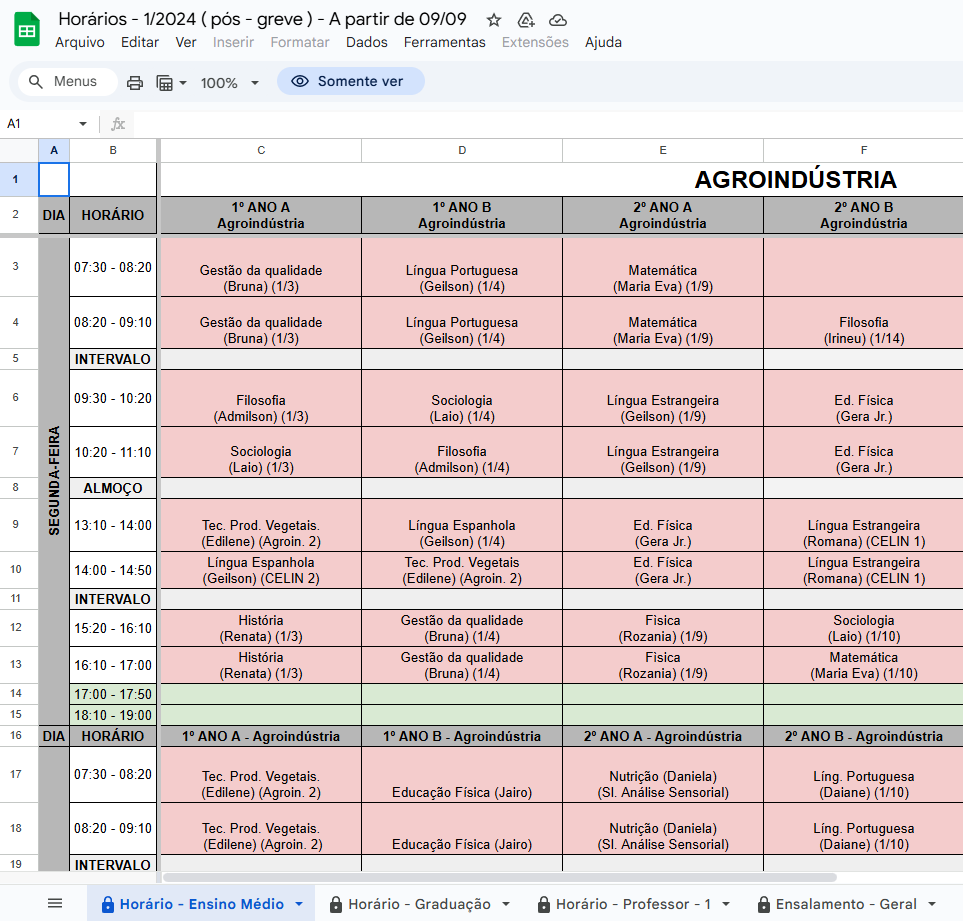
\includegraphics[width=0.9\textwidth]{figuras/plan-ant-1.png}
        \footnotesize Fonte: Elaborado pelo autor (2024)
    \end{minipage}
    \hfill
    \begin{minipage}{0.48\textwidth}
        \centering
        \captionof{figure}{Guia ``Horário - Graduação''}
        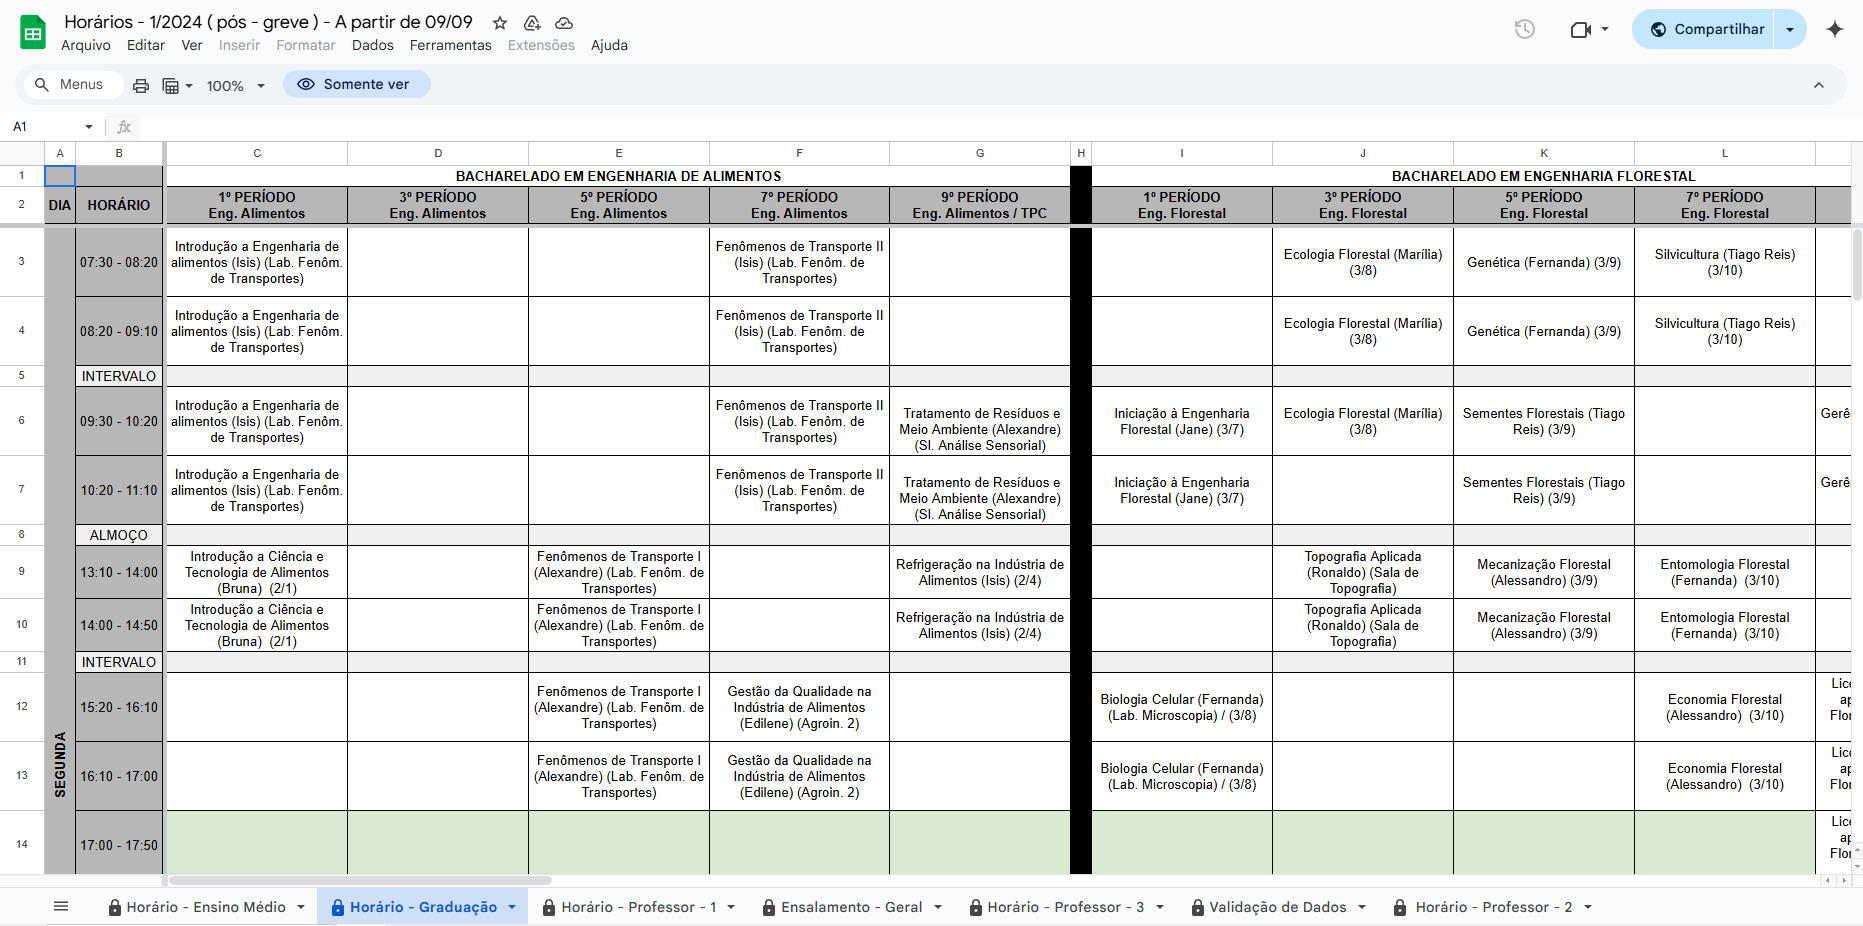
\includegraphics[width=0.9\textwidth]{figuras/plan-ant-2.png}
        \footnotesize Fonte: Elaborado pelo autor (2024)
    \end{minipage}
\end{frame}

\begin{frame}{Levantamento de Requisitos}
    \begin{itemize}
        \item Documentação: \vspace{0.5cm}
              \begin{enumerate}
                  \setcounter{enumi}{2}
                  \item Solução proposta; \vspace{0.5cm}
                  \item Funcionalidades desejadas. \vspace{0.5cm}
              \end{enumerate}
    \end{itemize}
\end{frame}

\begin{frame}{Front-end}
    \begin{itemize}
        \item Protótipo: \vspace{0.5cm}
              \begin{itemize}
                  \item Figma; \vspace{0.5cm}
              \end{itemize}
        \item Desenvolvimento: \vspace{0.5cm}
              \begin{itemize}
                  \item Next.js; \vspace{0.5cm}
                  \item Tailwind CSS. \vspace{0.5cm}
              \end{itemize}
        \item Justificativa. \vspace{0.5cm}
    \end{itemize}
\end{frame}

\begin{frame}{Back-end}
    \begin{itemize}
        \item Google Sheets como banco de dados: \vspace{0.5cm}
              \begin{itemize}
                  \item Benefícios; \vspace{0.5cm}
                  \item Processo de Atualização dos Dados: \vspace{0.5cm}
                        \begin{itemize}
                            \item O setor de ensino copia os dados mais recentes de uma planilha privada; \vspace{0.5cm}
                            \item Os dados são colados na planilha utilizada como banco de dados. \vspace{0.5cm}
                        \end{itemize}
              \end{itemize}
    \end{itemize}
\end{frame}

\begin{frame}{Back-end}
    \begin{itemize}
        \item Implementação: \vspace{0.5cm}
              \begin{itemize}
                  \item Spring Boot: \vspace{0.5cm}
                        \begin{itemize}
                            \item Essencial para estabelecer a conexão com a API do Google Sheets; \vspace{0.5cm}
                            \item Para garantir a segurança, configurada para permitir apenas operações de leitura. \vspace{0.5cm}
                        \end{itemize}
              \end{itemize}
        \item Arquitetura; \vspace{0.5cm}
        \item Justificativa. \vspace{0.5cm}
    \end{itemize}
\end{frame}

\begin{frame}{Integração Front-end com Back-end}
    \begin{itemize}
        \item Por meio de uma API RESTful; \vspace{0.5cm}
        \item Envio e retorno de dados; \vspace{0.5cm}
        \item Alterações feitas no Google Sheets apareceram automaticamente na plataforma; \vspace{0.5cm}
        \item Segurança e controle de acesso. \vspace{0.5cm}
    \end{itemize}
\end{frame}

\begin{frame}{Deploy}
    \begin{itemize}
        \item Front-end: Vercel; \vspace{0.5cm}
        \begin{itemize}
            \item Plataforma especializada no deploy de aplicações web baseadas em JavaScript. \vspace{0.5cm}
        \end{itemize}
        \item Back-end: Koyeb; \vspace{0.5cm}
        \begin{itemize}
            \item Plataforma serverless amigável para desenvolvedores. \vspace{0.5cm}
        \end{itemize}
    \end{itemize}
\end{frame}

\begin{frame}{Armazenamento do Código e Integração}
    \begin{itemize}
        \item Github; \vspace{0.5cm}
        \begin{itemize}
            \item Repositório de hospedagem de serviços Git. \vspace{0.5cm}
        \end{itemize}
        \item Conta vinculada com plataformas de deploy: \vspace{0.5cm}
              \begin{itemize}
                  \item Uso do Docker; \vspace{0.5cm}
              \end{itemize}
    \end{itemize}
\end{frame}

\begin{frame}{Ambiente de Desenvolvimento}
    \begin{itemize}
        \item Visual Studio Code; \vspace{0.5cm}
        \begin{itemize}
            \item Editor de código-fonte para auxiliar programadores na criação de softwares. \vspace{0.5cm}
        \end{itemize}
        \item Justificativa. \vspace{0.5cm}
    \end{itemize}
\end{frame}

\begin{frame}{Avaliação da Plataforma}
    \begin{itemize}
        \item Para avaliar a eficácia da plataforma; \vspace{0.5cm}
        \item Participação: Coordenador de Ensino Superior. \vspace{0.5cm}
    \end{itemize}
\end{frame}

\begin{frame}{Avaliação da Plataforma}
    \begin{itemize}
        \item A condução da entrevista foi realizada conforme os seguintes passos: \vspace{0.5cm}
              \begin{itemize}
                  \item Preparação: \vspace{0.5cm}
                        \begin{itemize}
                            \item Agendamento; \vspace{0.25cm}
                            \item Objetivos. \vspace{0.5cm}
                        \end{itemize}
                  \item Entrevista; \vspace{0.5cm}
                  \item Perguntas; \vspace{0.25cm}
                  \begin{itemize}
                    \item Com base no instrumento do TCC: ``SIGALAB: Sistema de Informação Gerencial Acadêmico para Reservas de Laboratórios''.
                  \end{itemize}
              \end{itemize}
    \end{itemize}
\end{frame}

\begin{frame}{Avaliação da Plataforma}
    \begin{itemize}
        \item Documentação: \vspace{0.5cm}
              \begin{enumerate}
                  \item Usabilidade e navegação; \vspace{0.5cm}
                  \item Eficiência na exibição dos horários; \vspace{0.5cm}
                  \item Redução de dificuldades operacionais; \vspace{0.5cm}
                  \item Satisfação geral; \vspace{0.5cm}
                  \item Melhorias e atualizações; \vspace{0.5cm}
                  \item Garantia de disponibilidade. \vspace{0.5cm}
              \end{enumerate}
    \end{itemize}
\end{frame}

\begin{frame}{Implementação de Melhorias e Atualizações}
    \begin{itemize}
        \item O histórico das versões desenvolvidas até o momento: \vspace{0.5cm}
              \begin{itemize}
                  \item v.1.0.0; \vspace{0.5cm}
                  \item v.2.0.0. \vspace{0.25cm}
                  \begin{itemize}
                    \item Criação de uma nova planilha no Google Sheets com as credenciais de login para acessar a tela de validação de dados; \vspace{0.25cm}
                    \item Implementação de uma nova tela para a validação dos dados da planilha dos horários; \vspace{0.25cm}
                    \item Adição de um botão no menu principal da plataforma para direcionar para validação de dados; \vspace{0.25cm}
                    \item Inclusão de três novos botões no menu principal da plataforma com links externos para os sistemas complementares. \vspace{0.25cm}
                  \end{itemize}
              \end{itemize}
    \end{itemize}
\end{frame}

\begin{frame}{Documentação}
    \begin{itemize}
        \item Para garantir a correta manutenção e funcionamento da plataforma; \vspace{0.5cm}
        \item Abordou os seguintes aspectos: \vspace{0.5cm}
              \begin{itemize}
                  \item Estrutura e organização dos dados; \vspace{0.5cm}
                  \item Regras para adição e atualização de informações; \vspace{0.5cm}
                  \item Padrões para nomes de guias e intervalos de células.
              \end{itemize}
    \end{itemize}
\end{frame}

\section{Resultados}

\begin{frame}{Resultados}
    \begin{itemize}
		\item Front-end: Protótipos \vspace{0.5cm}
	\end{itemize}
    \begin{figure}
        \centering
        \vspace{-0.8cm}
        \caption{Protótipo da tela inicial}
        \vspace{-0.2cm}
        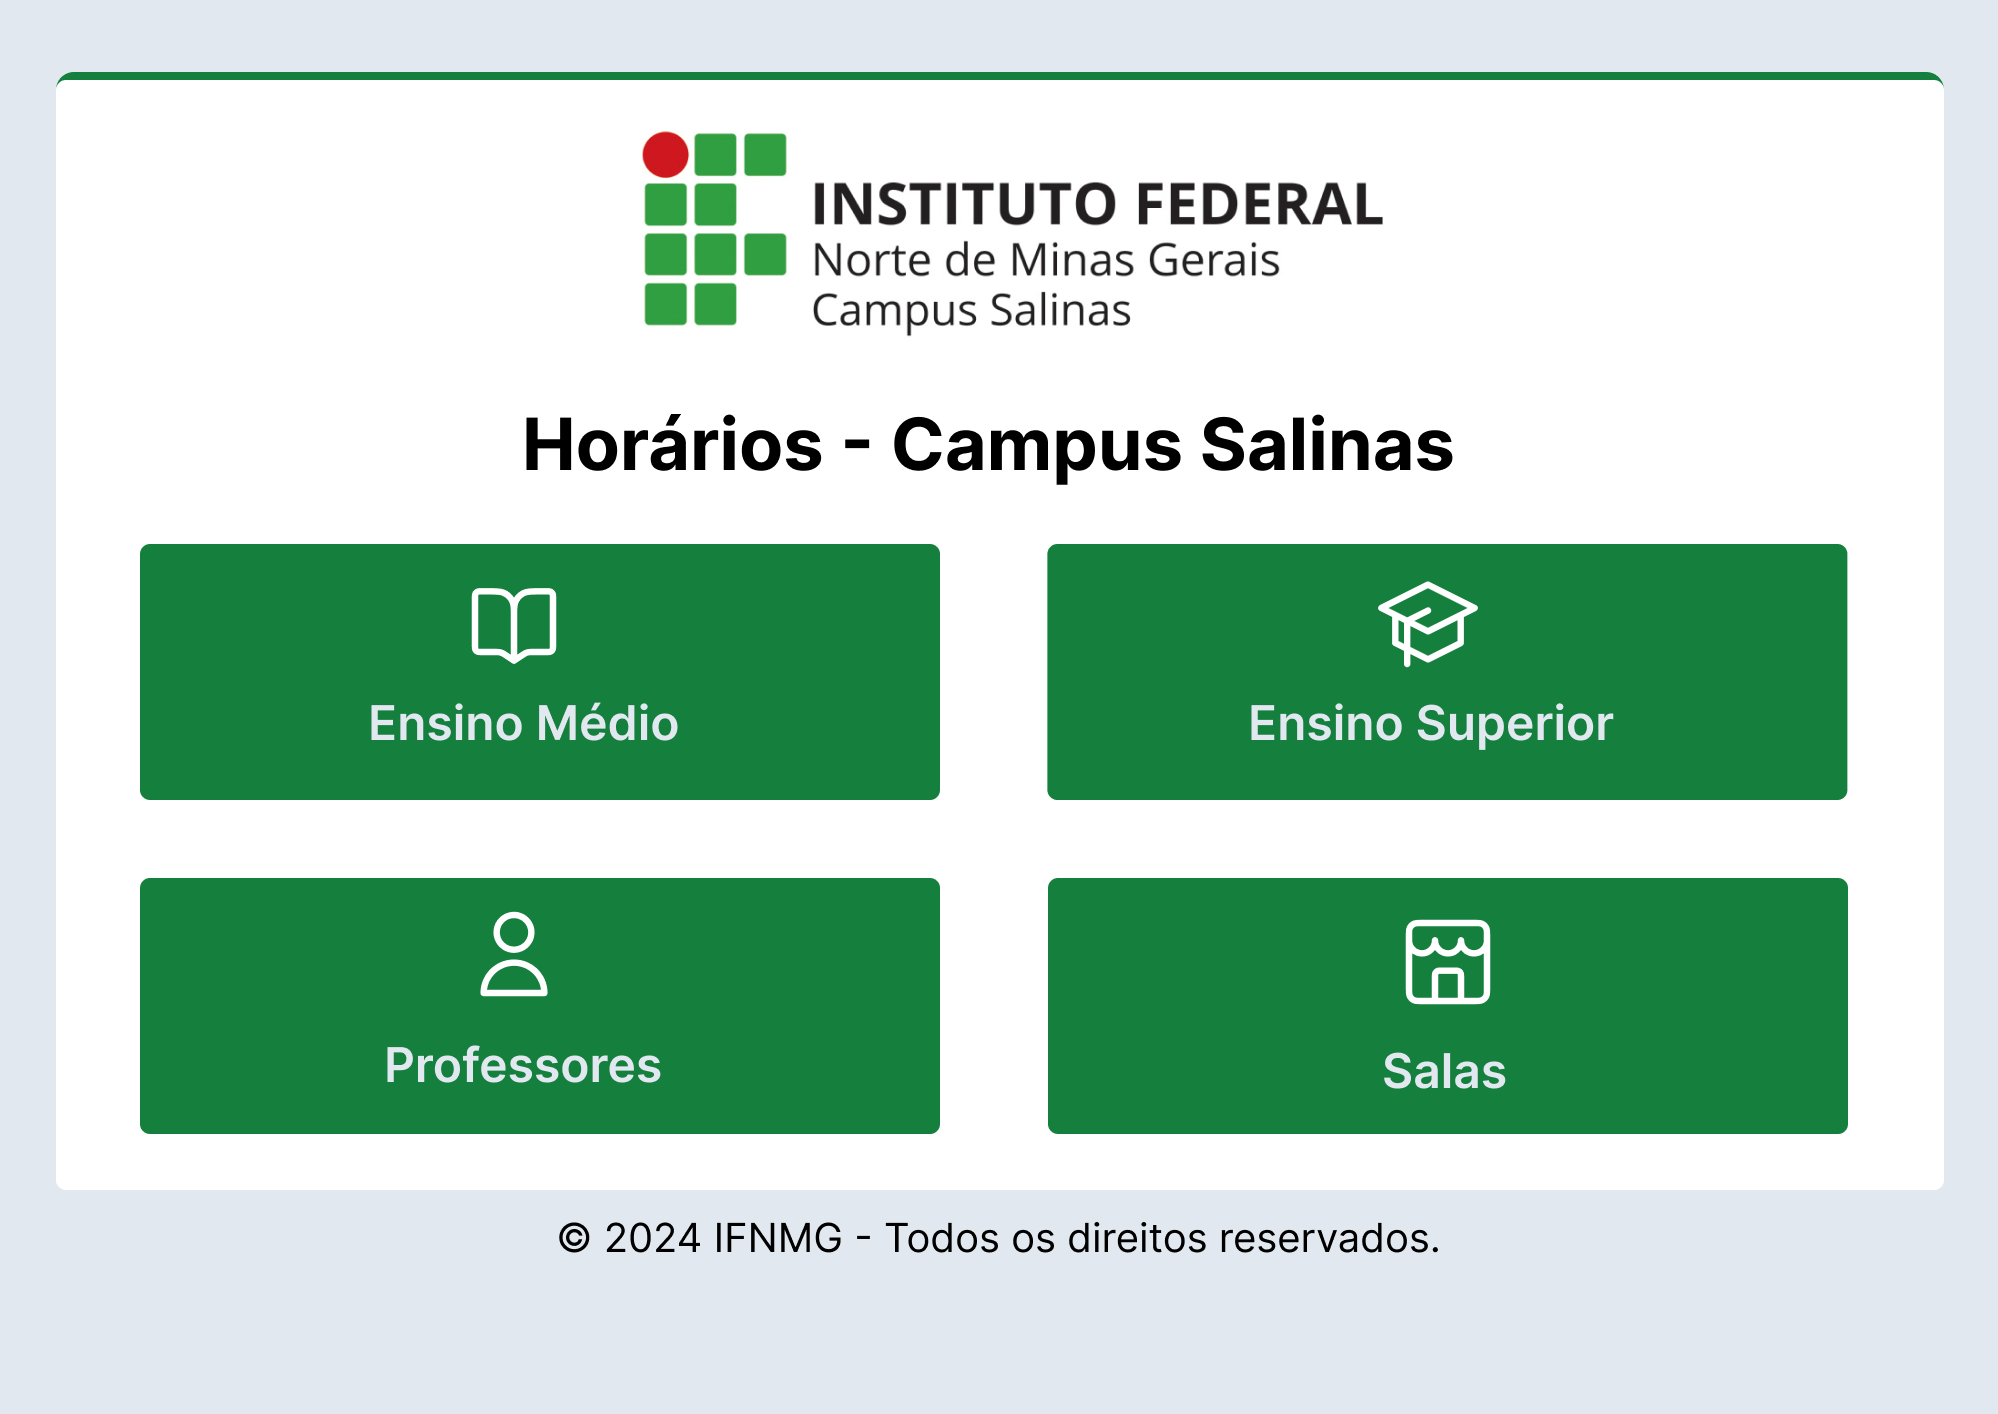
\includegraphics[width=0.7\textwidth]{figuras/proto-1.png}
        \\ % Quebra de linha para separar a imagem da fonte
        \small Fonte: Elaborado pelo autor (2024)
    \end{figure}
\end{frame}

\begin{frame}{Protótipos}
    \begin{figure}
        \centering
        \vspace{-0.5cm}
        \caption{Protótipo da tela dos cursos}
        \vspace{-0.2cm}
        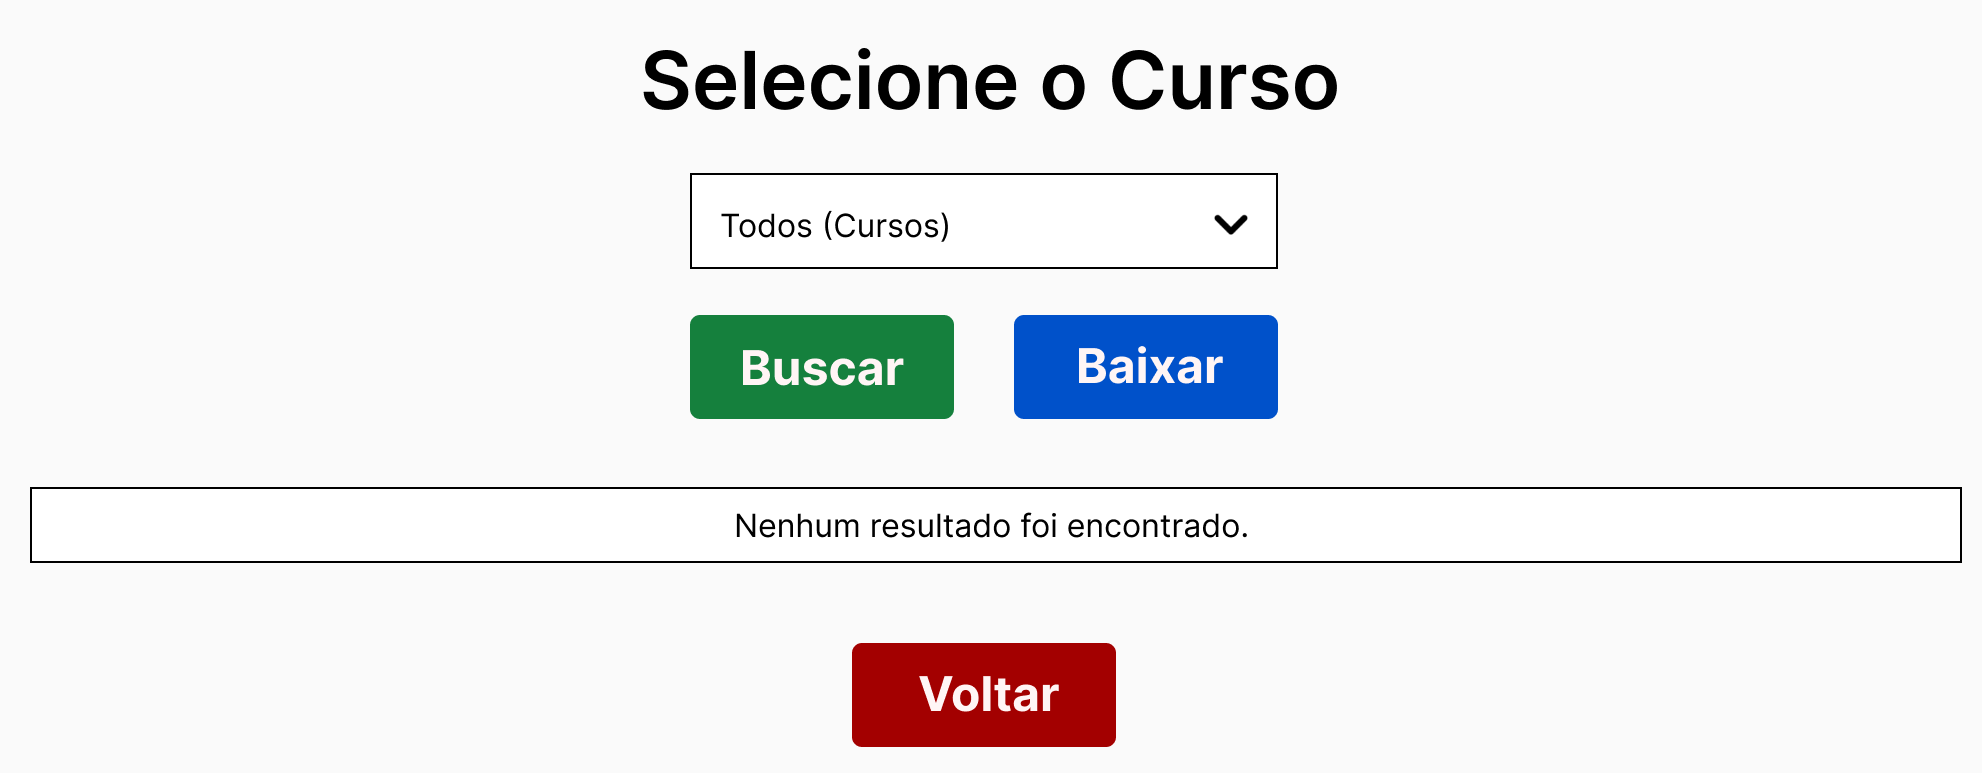
\includegraphics[width=0.7\textwidth]{figuras/proto-2.png}
        \\ % Quebra de linha para separar a imagem da fonte
        \small Fonte: Elaborado pelo autor (2024)
    \end{figure}
\end{frame}

\begin{frame}{Protótipos}
    \begin{figure}
        \centering
        \vspace{-0.5cm}
        \caption{Protótipo da tela dos cursos preenchida}
        \vspace{-0.2cm}
        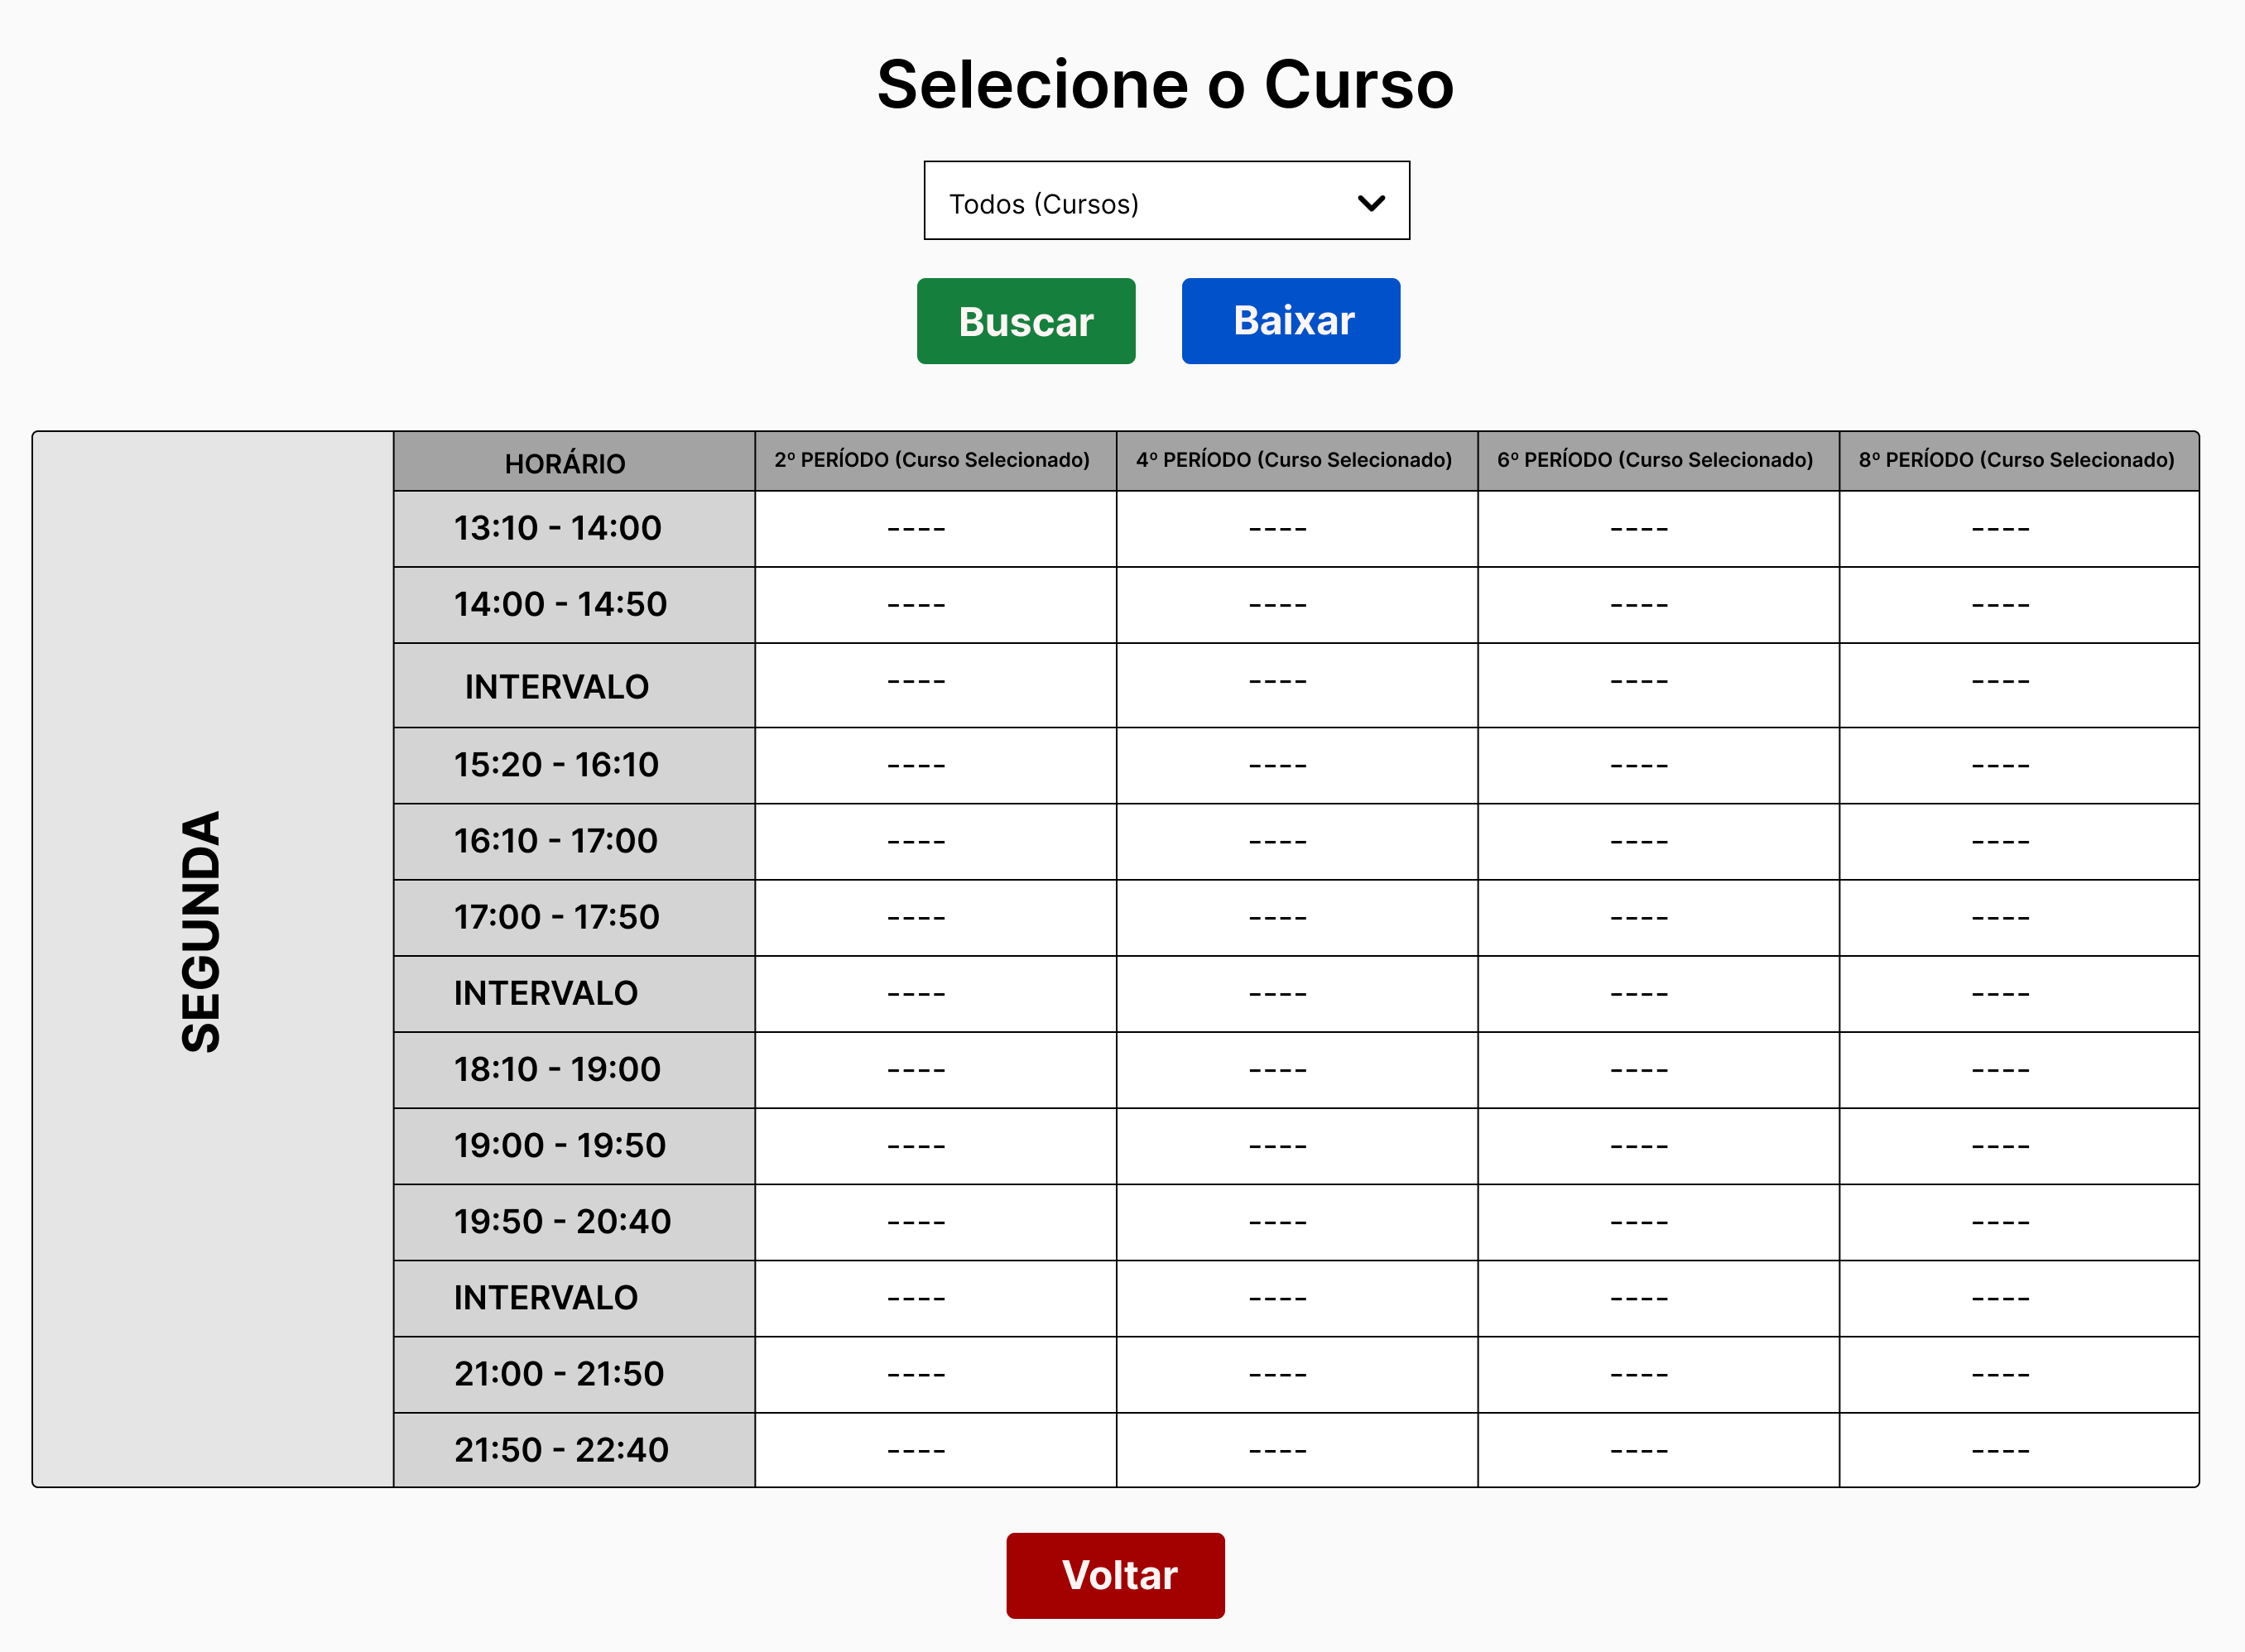
\includegraphics[width=0.7\textwidth]{figuras/proto-3.png}
        \\ % Quebra de linha para separar a imagem da fonte
        \small Fonte: Elaborado pelo autor (2024)
    \end{figure}
\end{frame}

\begin{frame}{Protótipos}
    \begin{figure}
        \centering
        \vspace{-0.5cm}
        \caption{Protótipo da tela dos professores}
        \vspace{-0.2cm}
        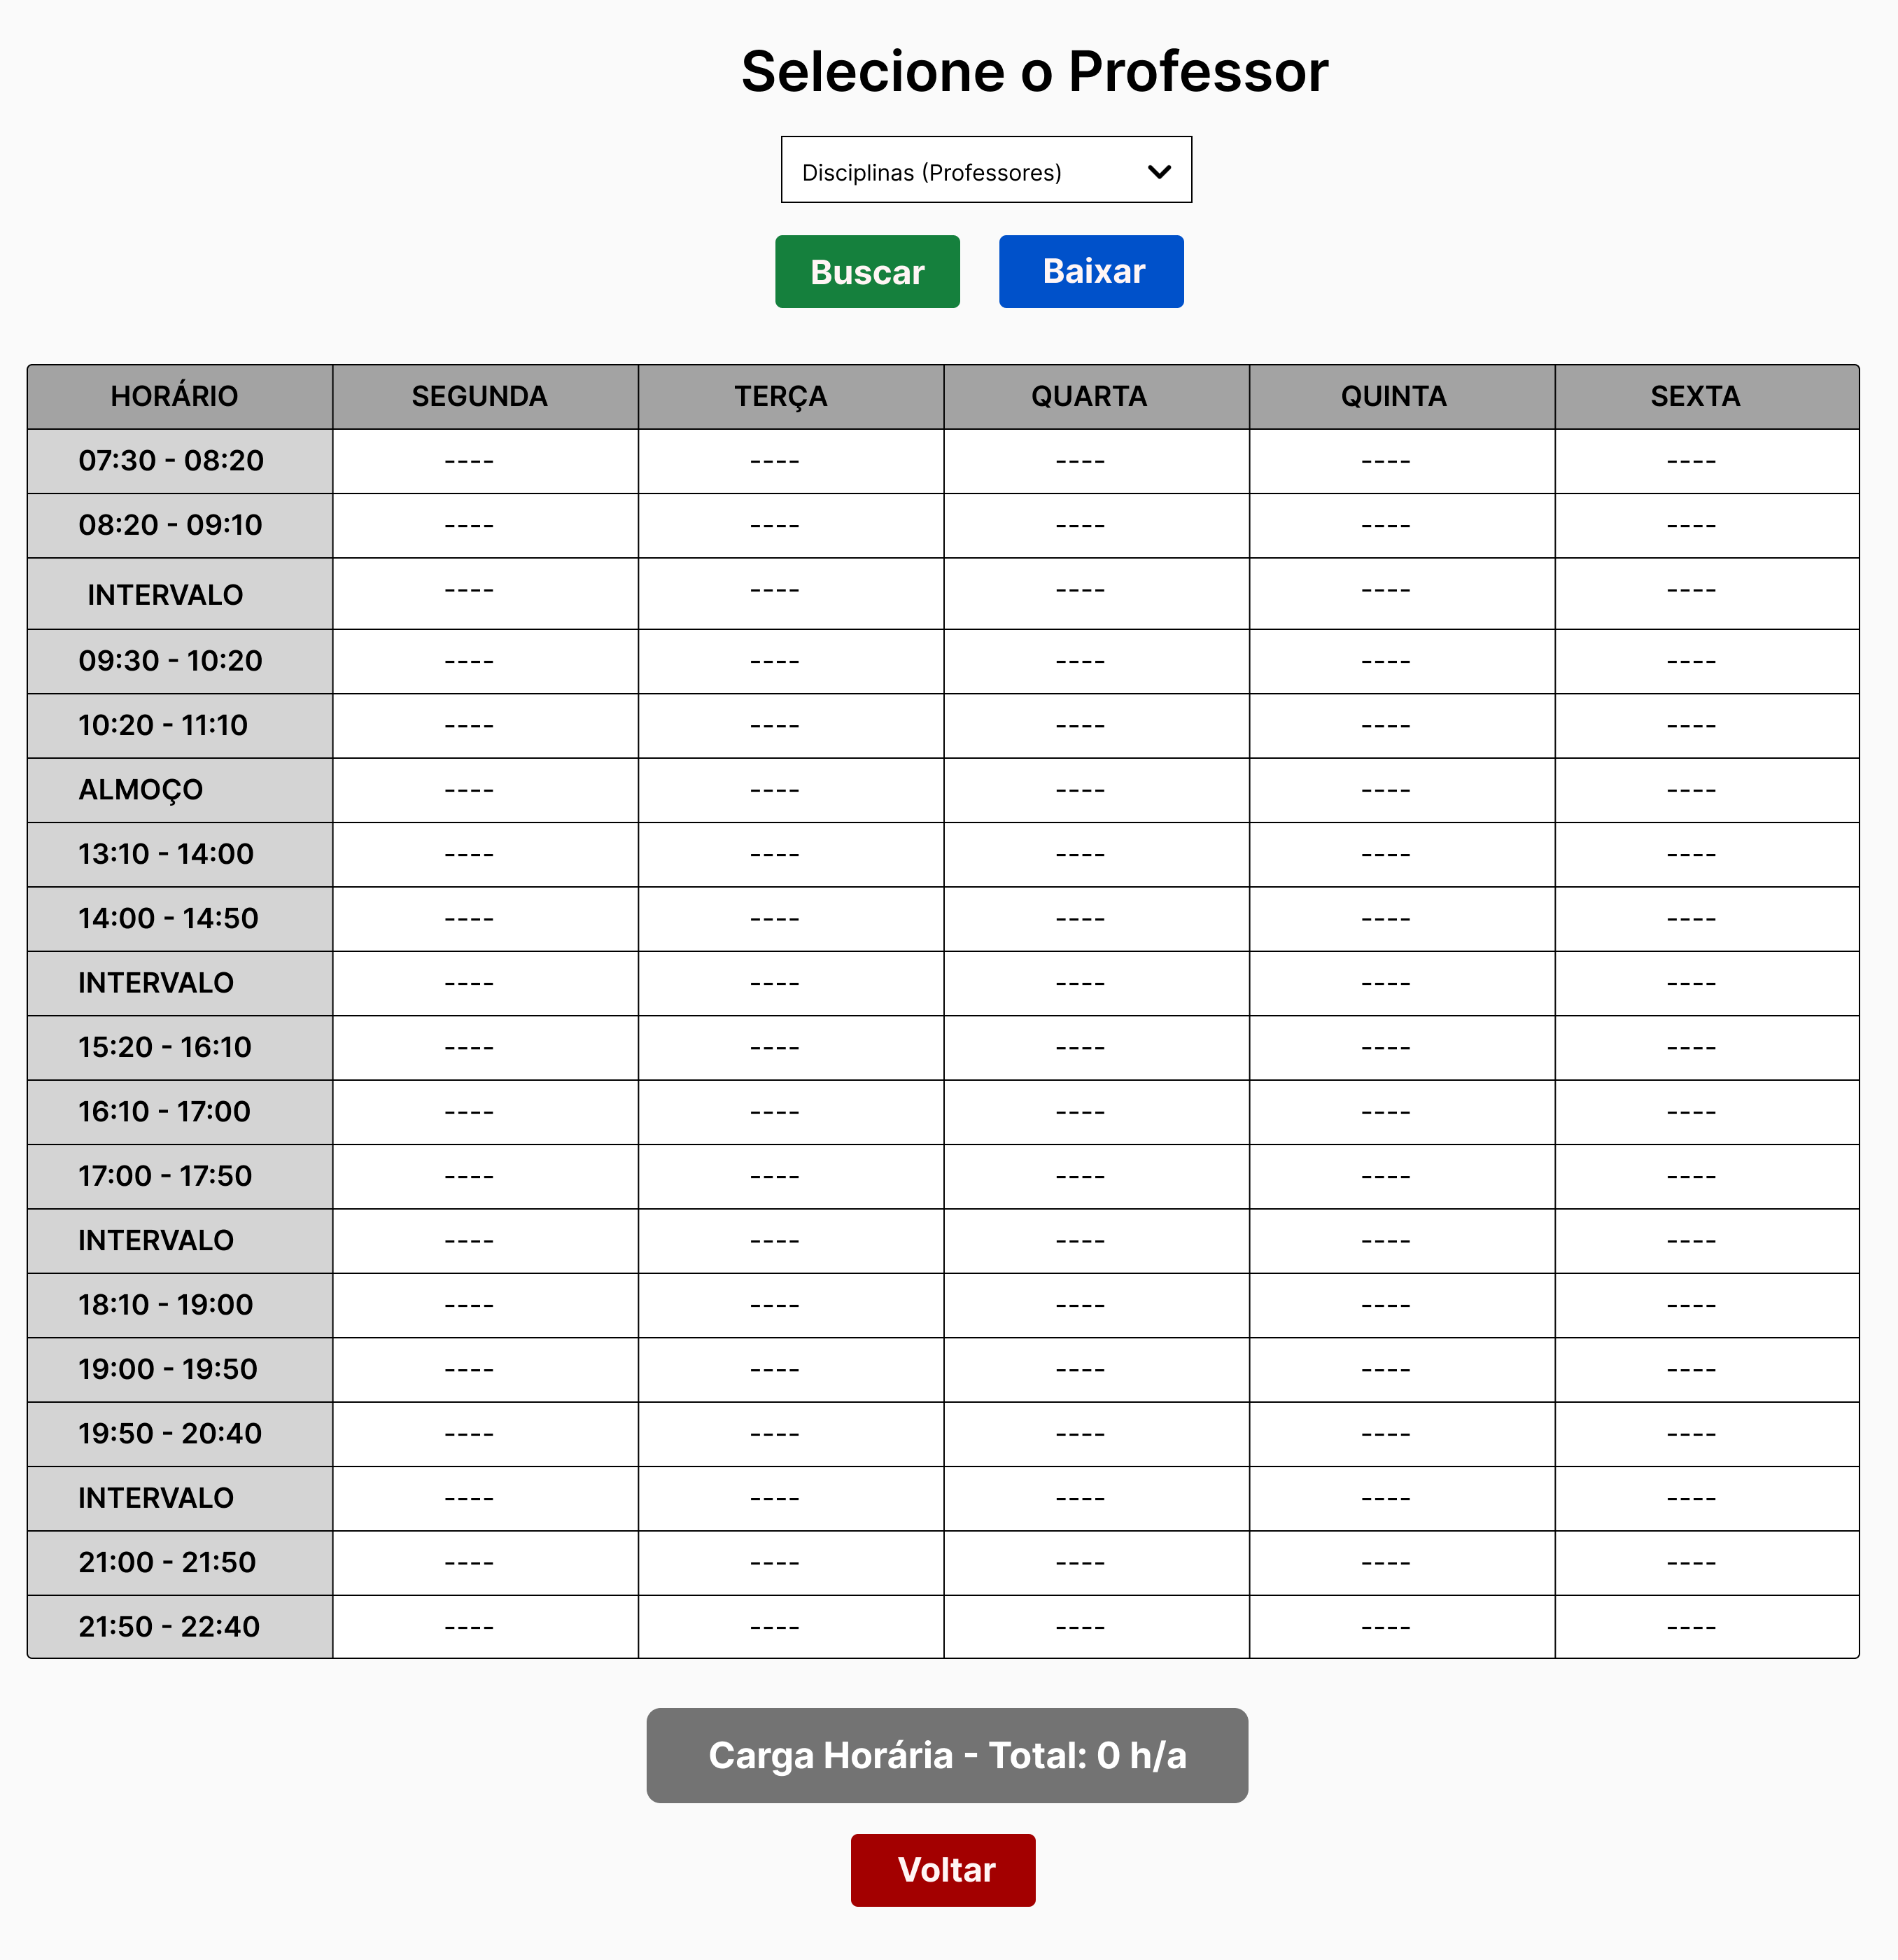
\includegraphics[width=0.5\textwidth]{figuras/proto-4.png}
        \\ % Quebra de linha para separar a imagem da fonte
        \small Fonte: Elaborado pelo autor (2024)
    \end{figure}
\end{frame}

\begin{frame}{Protótipos}
    \begin{figure}
        \centering
        \vspace{-0.5cm}
        \caption{Protótipo da tela das salas}
        \vspace{-0.2cm}
        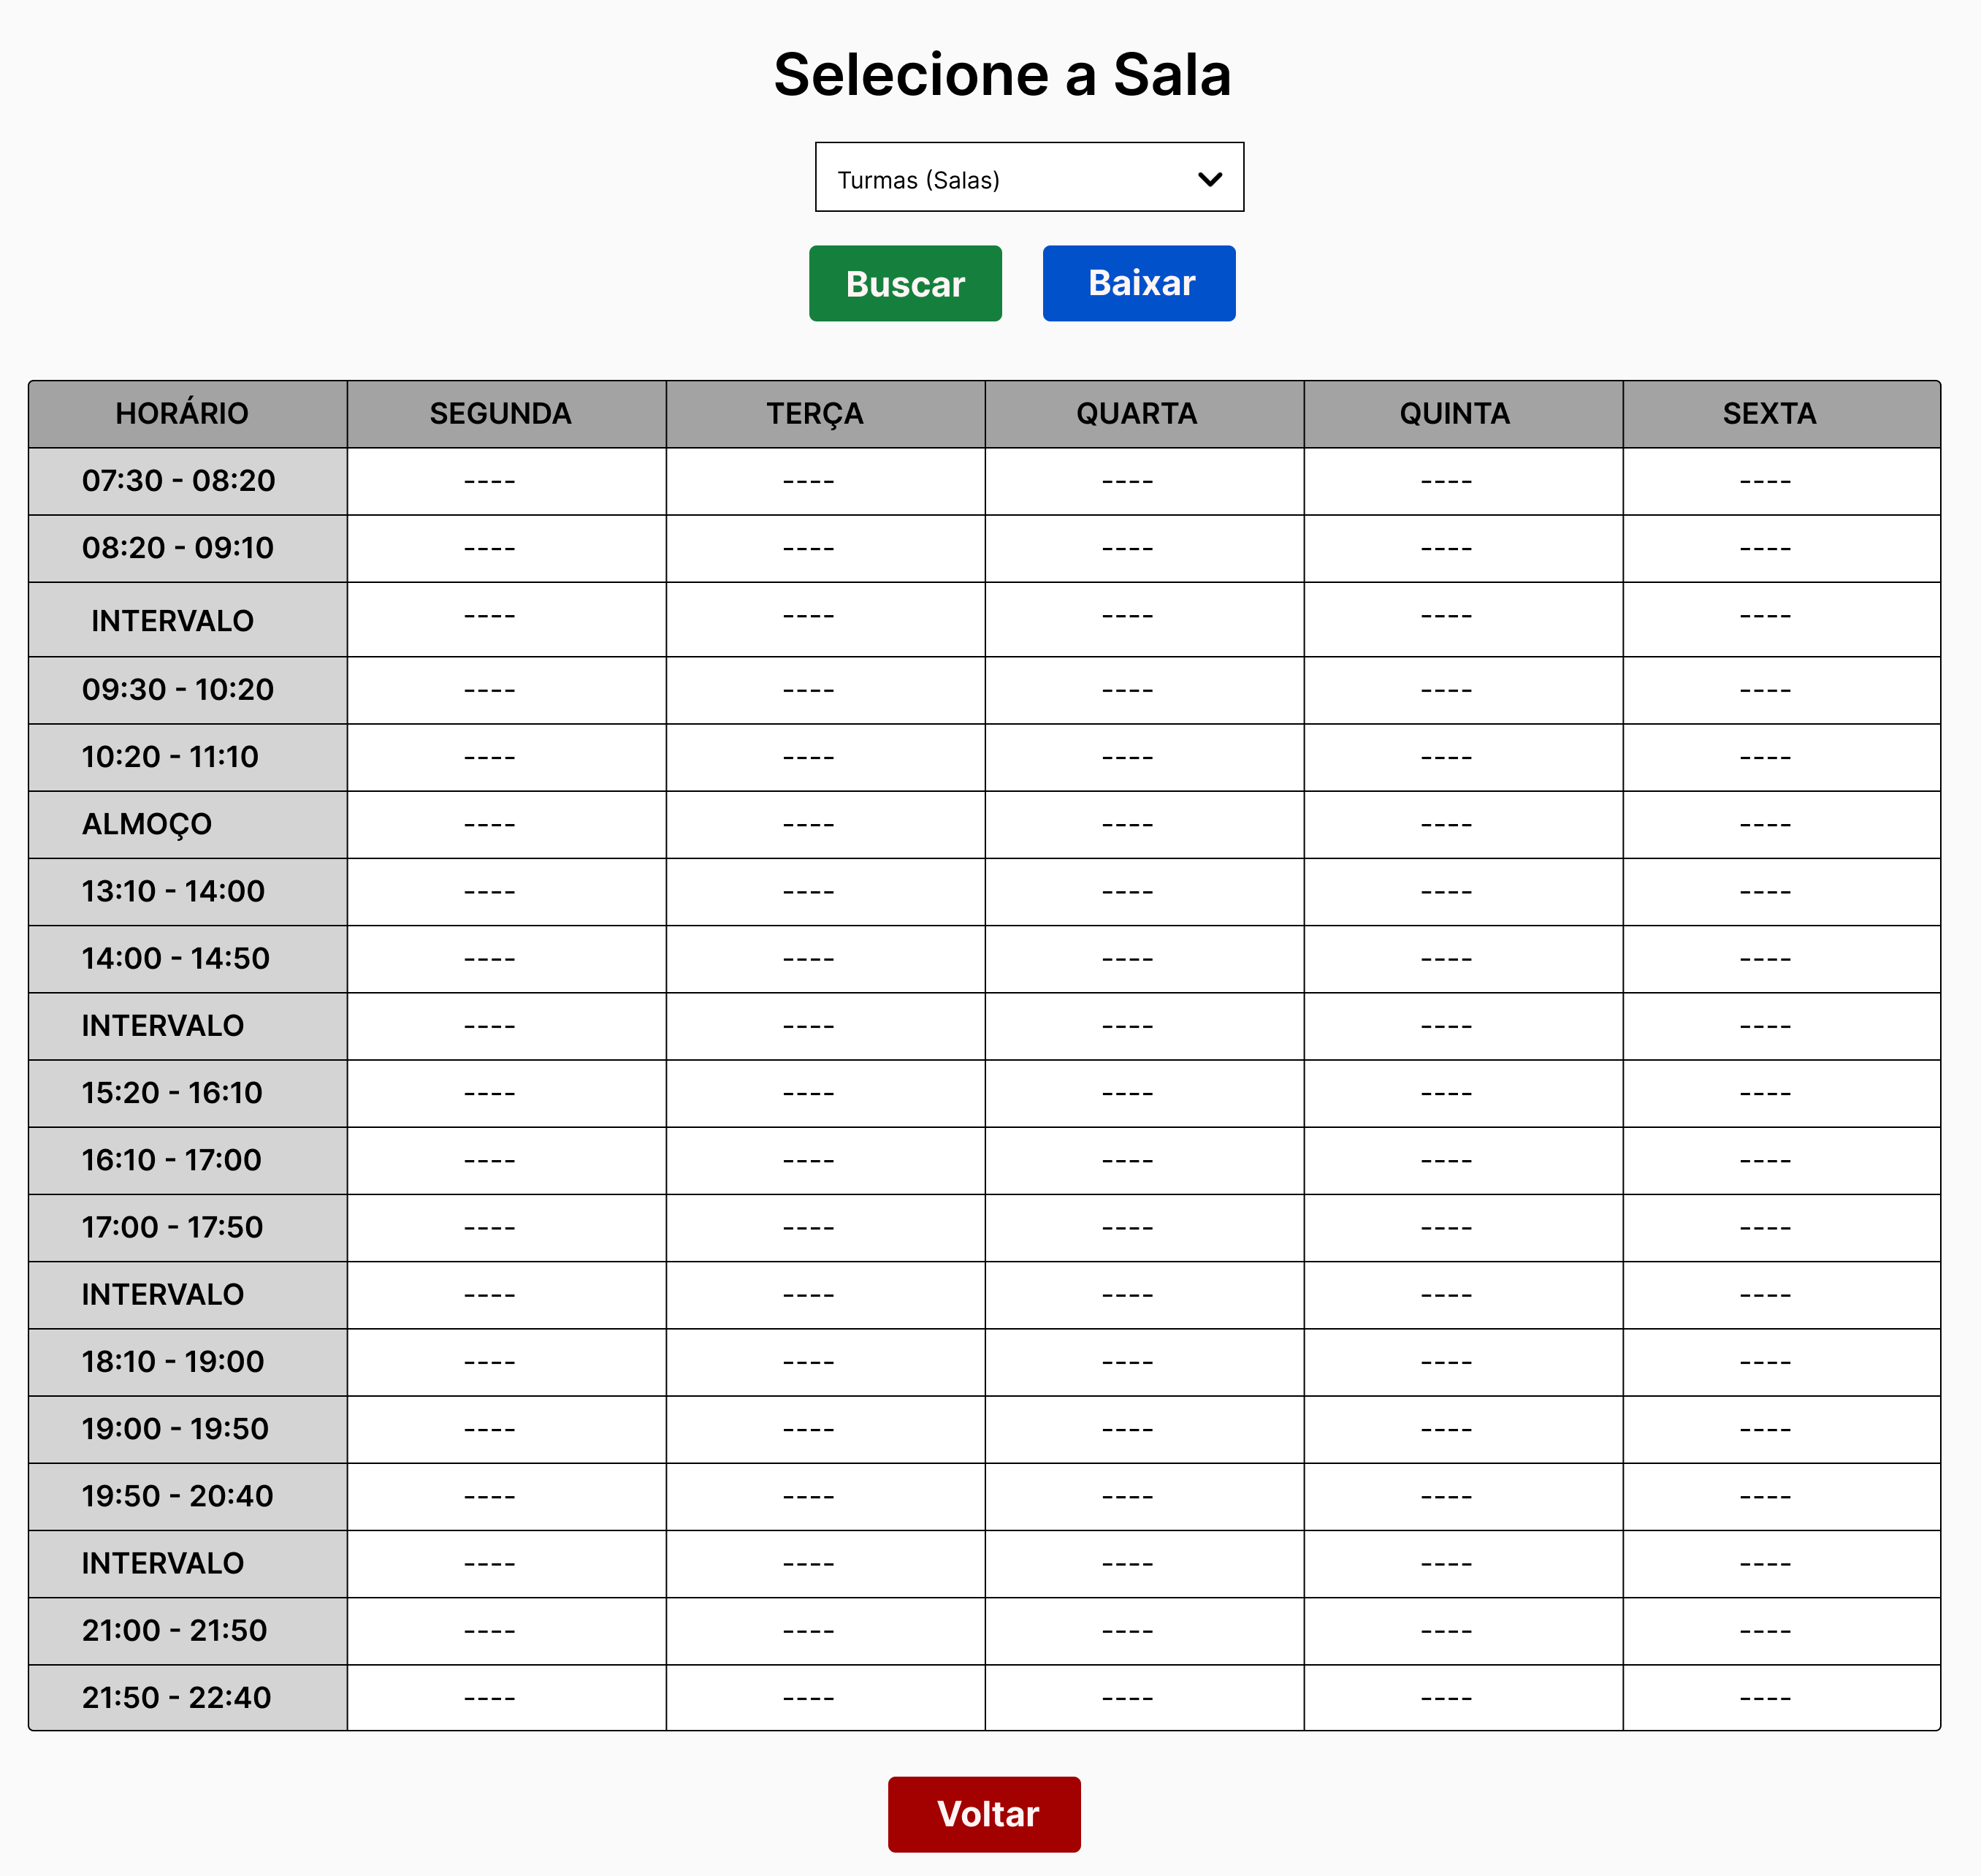
\includegraphics[width=0.5\textwidth]{figuras/proto-5.png}
        \\ % Quebra de linha para separar a imagem da fonte
        \small Fonte: Elaborado pelo autor (2024)
    \end{figure}
\end{frame}

\begin{frame}{Desenvolvimento do Front-end}
    \begin{figure}
        \centering
        \vspace{-0.5cm}
        \caption{Menu principal com opções de botões de horários e outros serviços}
        \vspace{-0.2cm}
        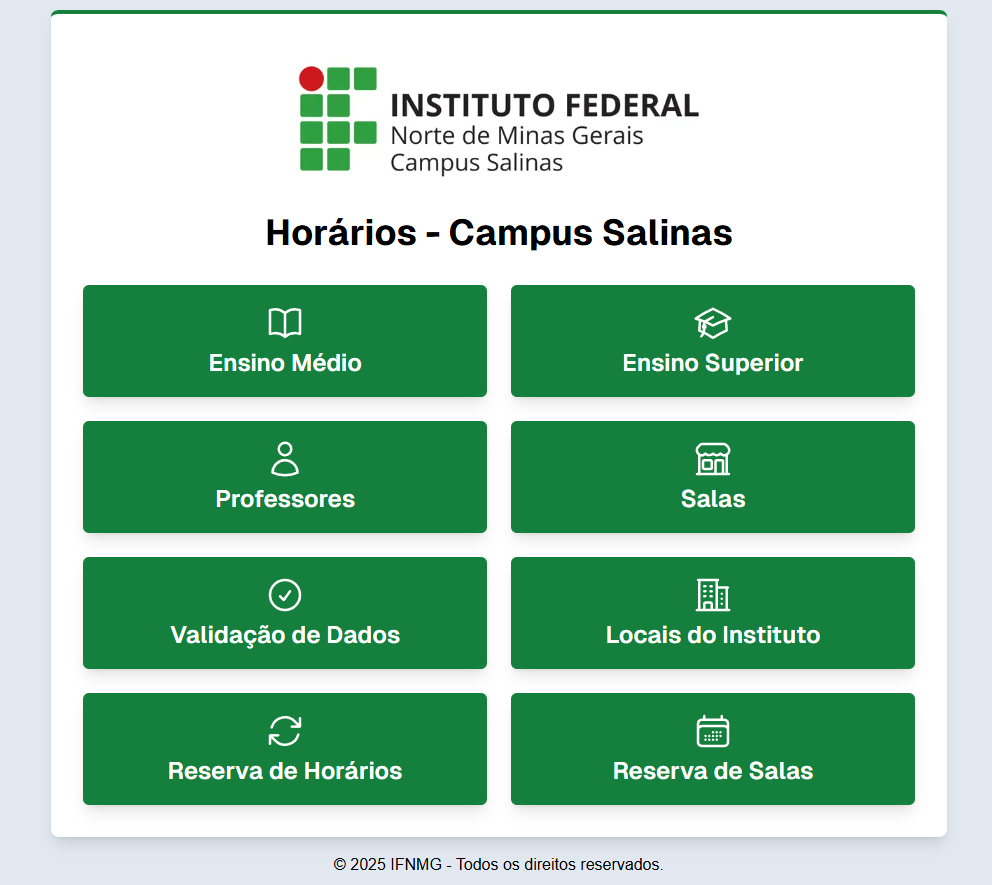
\includegraphics[width=0.5\textwidth]{figuras/front-1.png}
        \\ % Quebra de linha para separar a imagem da fonte
        \small Fonte: Elaborado pelo autor (2025)
    \end{figure}
\end{frame}

\begin{frame}{Desenvolvimento do Front-end}
    \begin{figure}
        \centering
        \vspace{-0.5cm}
        \caption{Tela dos cursos}
        \vspace{-0.2cm}
        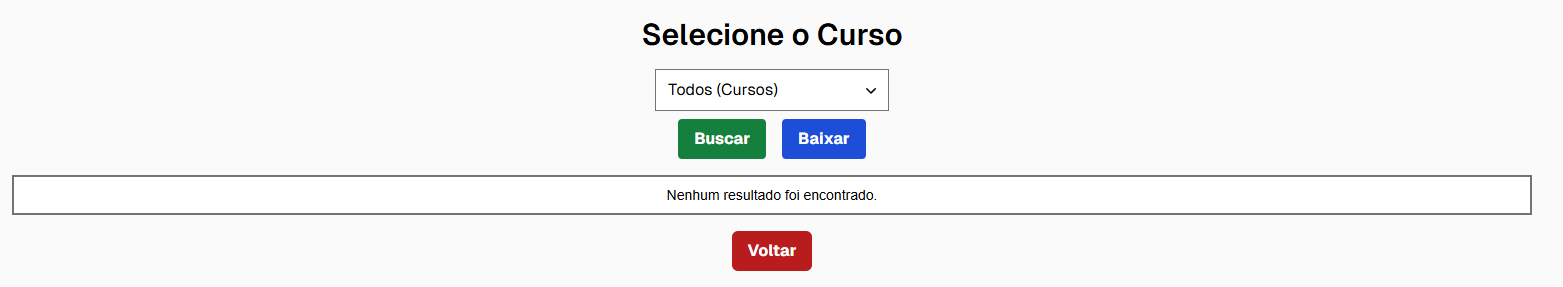
\includegraphics[width=0.8\textwidth]{figuras/front-2.png}
        \\ % Quebra de linha para separar a imagem da fonte
        \small Fonte: Elaborado pelo autor (2025)
    \end{figure}
\end{frame}

\begin{frame}{Desenvolvimento do Front-end}
    \begin{figure}
        \centering
        \vspace{-0.5cm}
        \caption{Tela dos cursos com cursos técnicos}
        \vspace{-0.2cm}
        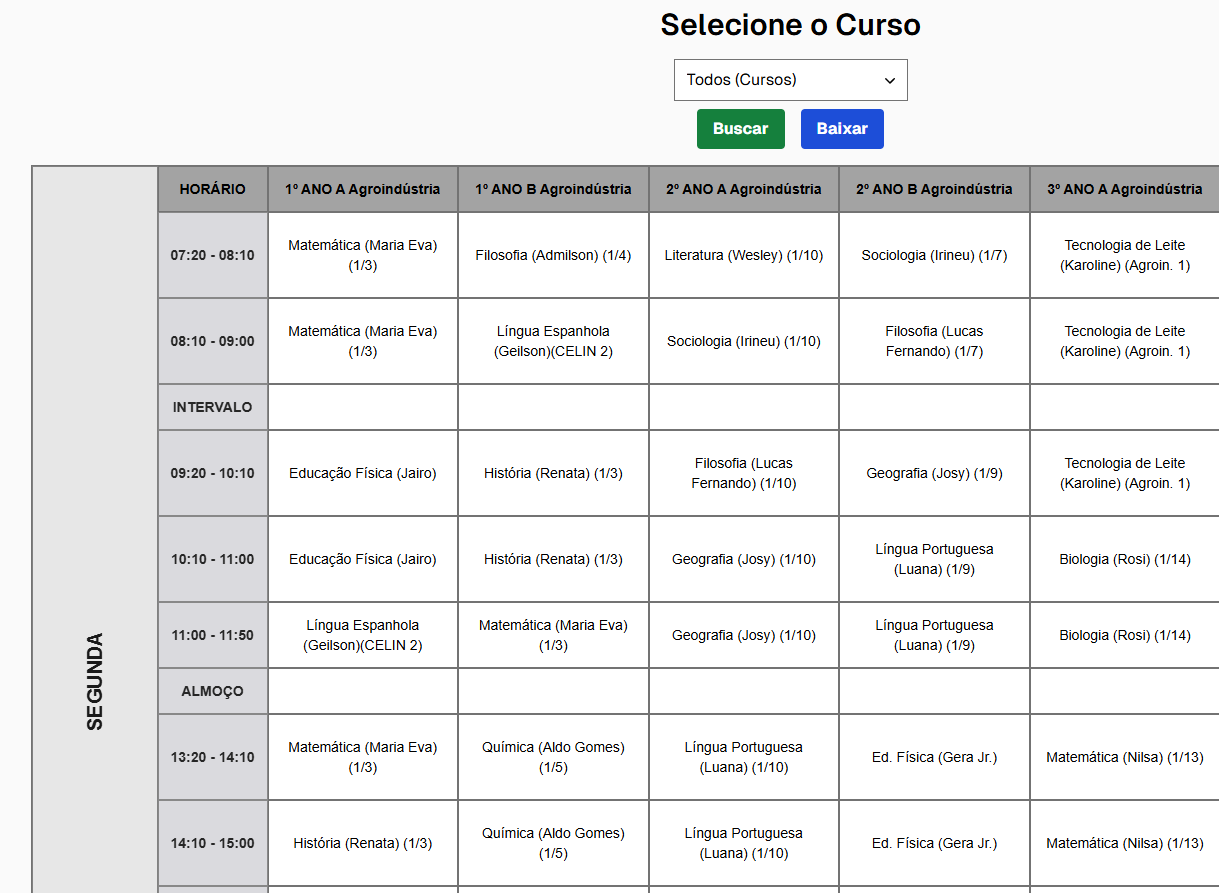
\includegraphics[width=0.8\textwidth]{figuras/front-3.png}
        \\ % Quebra de linha para separar a imagem da fonte
        \small Fonte: Elaborado pelo autor (2025)
    \end{figure}
\end{frame}

\begin{frame}{Desenvolvimento do Front-end}
    \begin{figure}
        \centering
        \vspace{-0.5cm}
        \caption{Tela dos cursos com cursos superiores}
        \vspace{-0.2cm}
        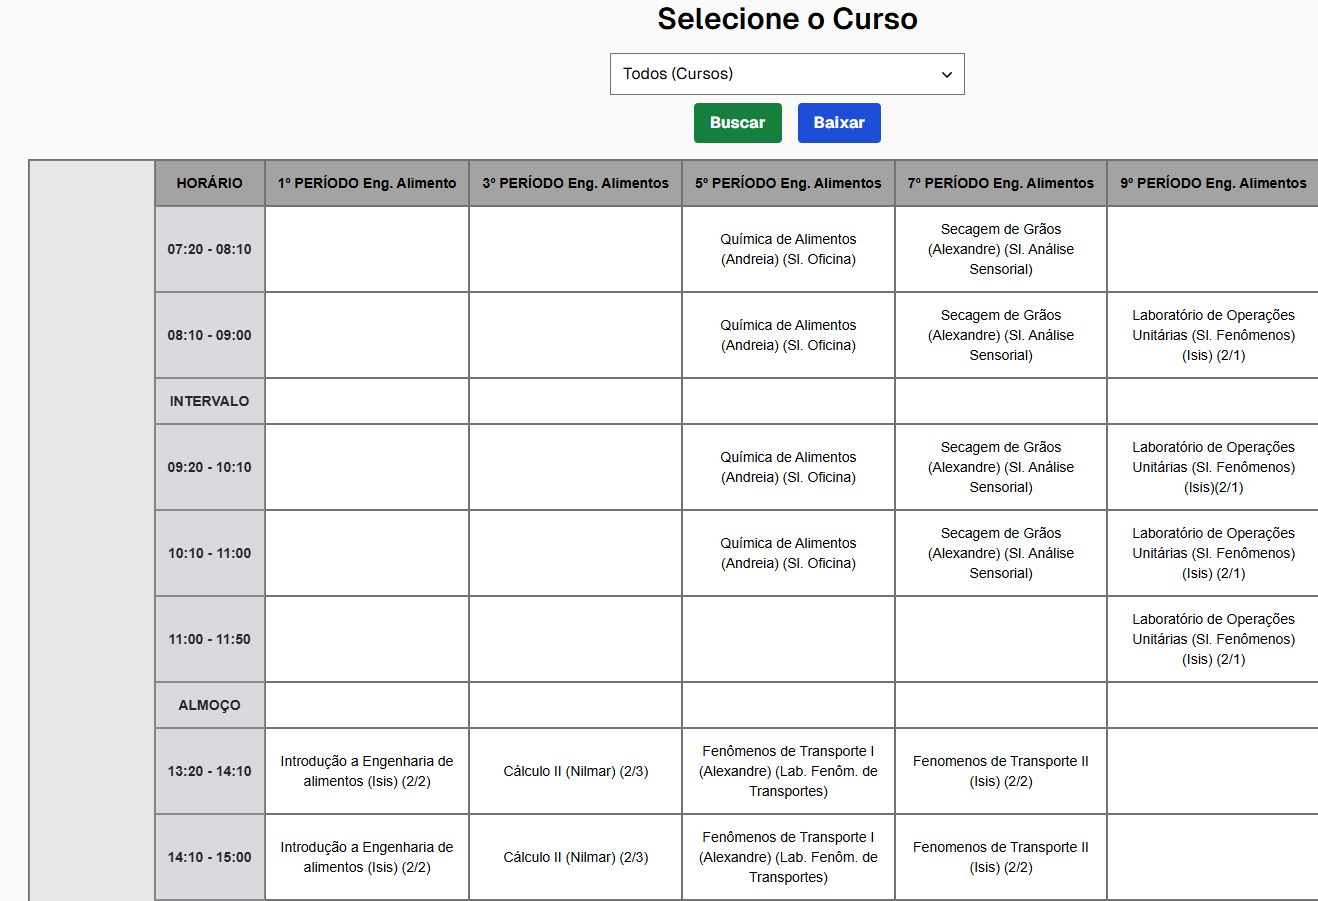
\includegraphics[width=0.8\textwidth]{figuras/front-4.png}
        \\ % Quebra de linha para separar a imagem da fonte
        \small Fonte: Elaborado pelo autor (2025)
    \end{figure}
\end{frame}

\begin{frame}{Desenvolvimento do Front-end}
    \begin{figure}
        \centering
        \vspace{-0.5cm}
        \caption{Tela dos professores}
        \vspace{-0.2cm}
        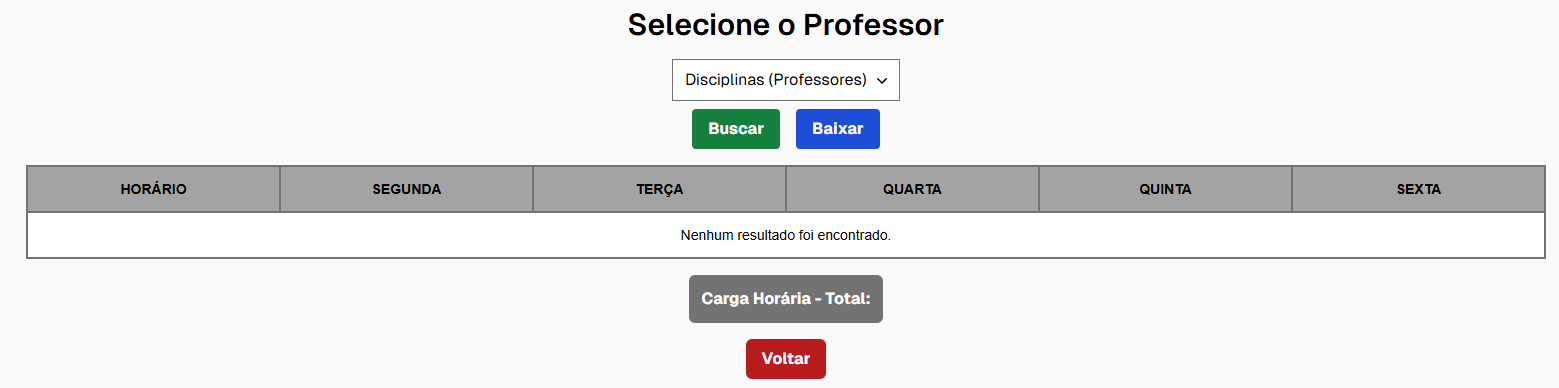
\includegraphics[width=0.8\textwidth]{figuras/front-5.png}
        \\ % Quebra de linha para separar a imagem da fonte
        \small Fonte: Elaborado pelo autor (2025)
    \end{figure}
\end{frame}

\begin{frame}{Desenvolvimento do Front-end}
    \begin{figure}
        \centering
        \vspace{-0.5cm}
        \caption{Tela dos professores com um professor selecionado}
        \vspace{-0.2cm}
        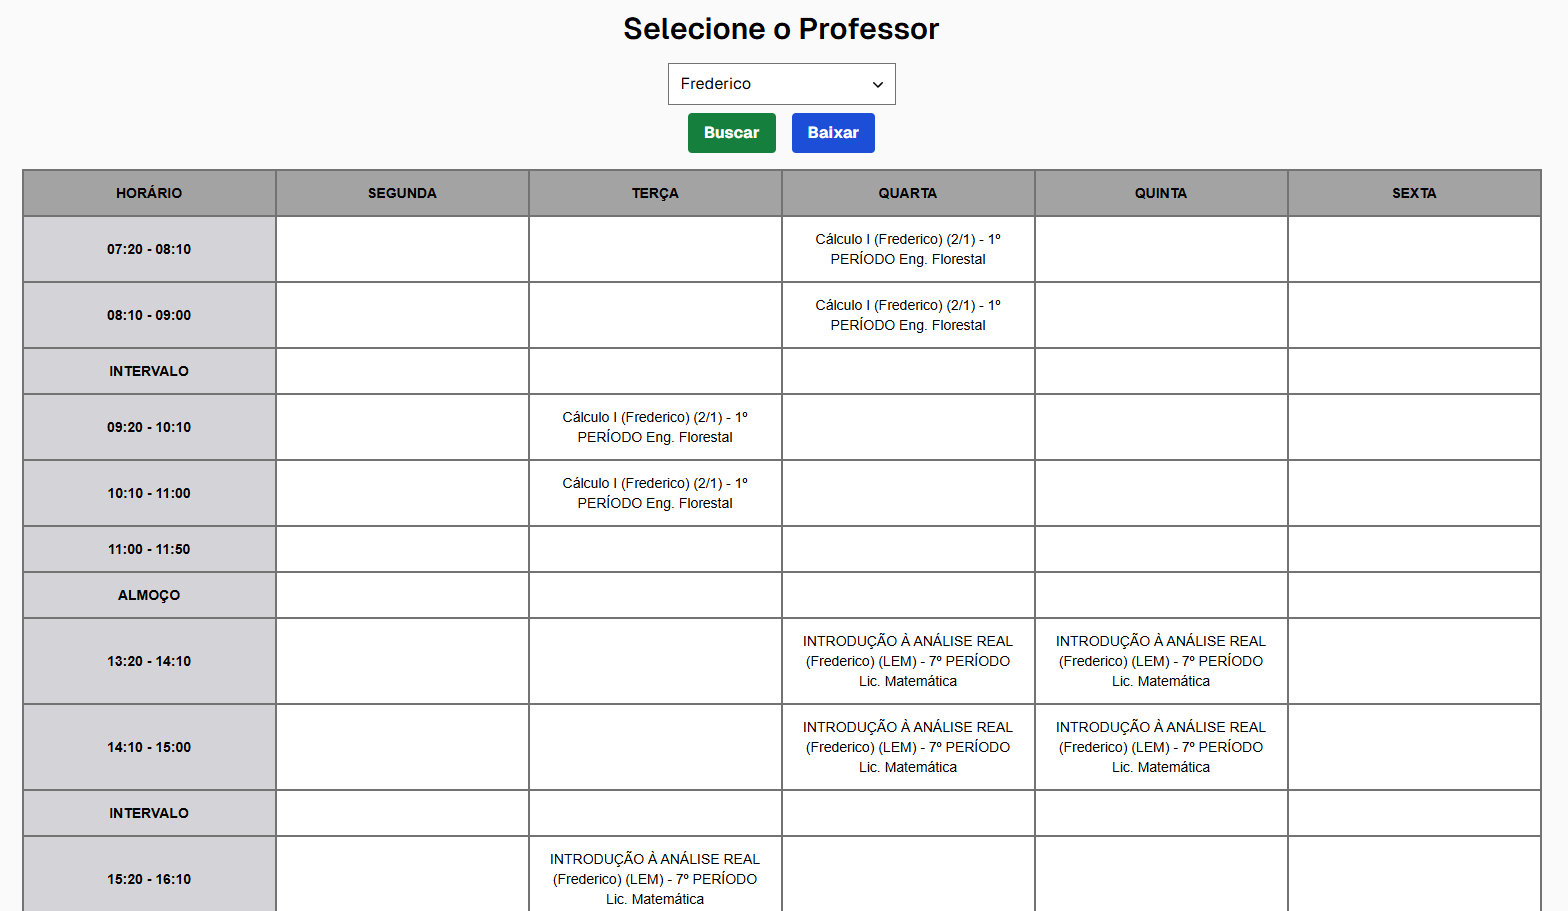
\includegraphics[width=0.8\textwidth]{figuras/front-6.png}
        \\ % Quebra de linha para separar a imagem da fonte
        \small Fonte: Elaborado pelo autor (2025)
    \end{figure}
\end{frame}

\begin{frame}{Desenvolvimento do Front-end}
    \begin{figure}
        \centering
        \vspace{-0.5cm}
        \caption{Tela das salas}
        \vspace{-0.2cm}
        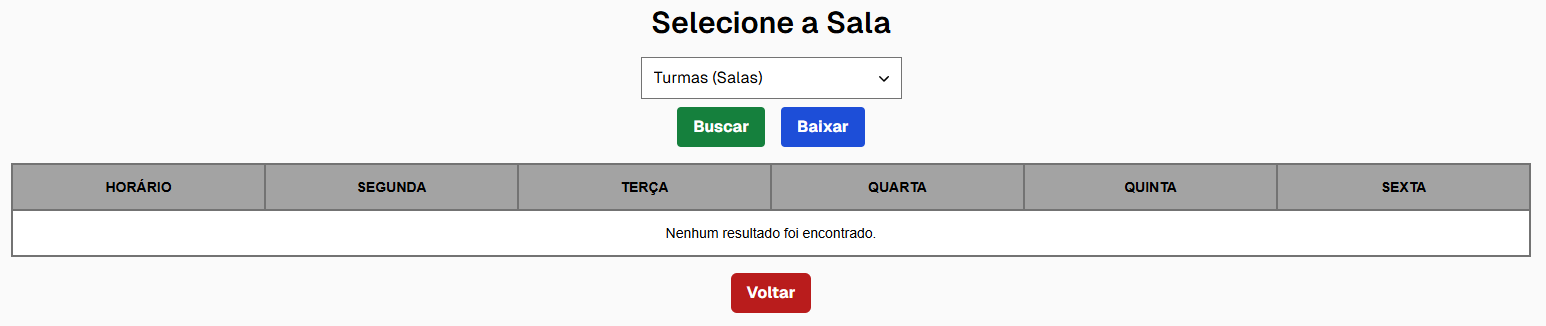
\includegraphics[width=0.8\textwidth]{figuras/front-7.png}
        \\ % Quebra de linha para separar a imagem da fonte
        \small Fonte: Elaborado pelo autor (2025)
    \end{figure}
\end{frame}

\begin{frame}{Desenvolvimento do Front-end}
    \begin{figure}
        \centering
        \vspace{-0.5cm}
        \caption{Tela das salas com uma sala selecionada}
        \vspace{-0.2cm}
        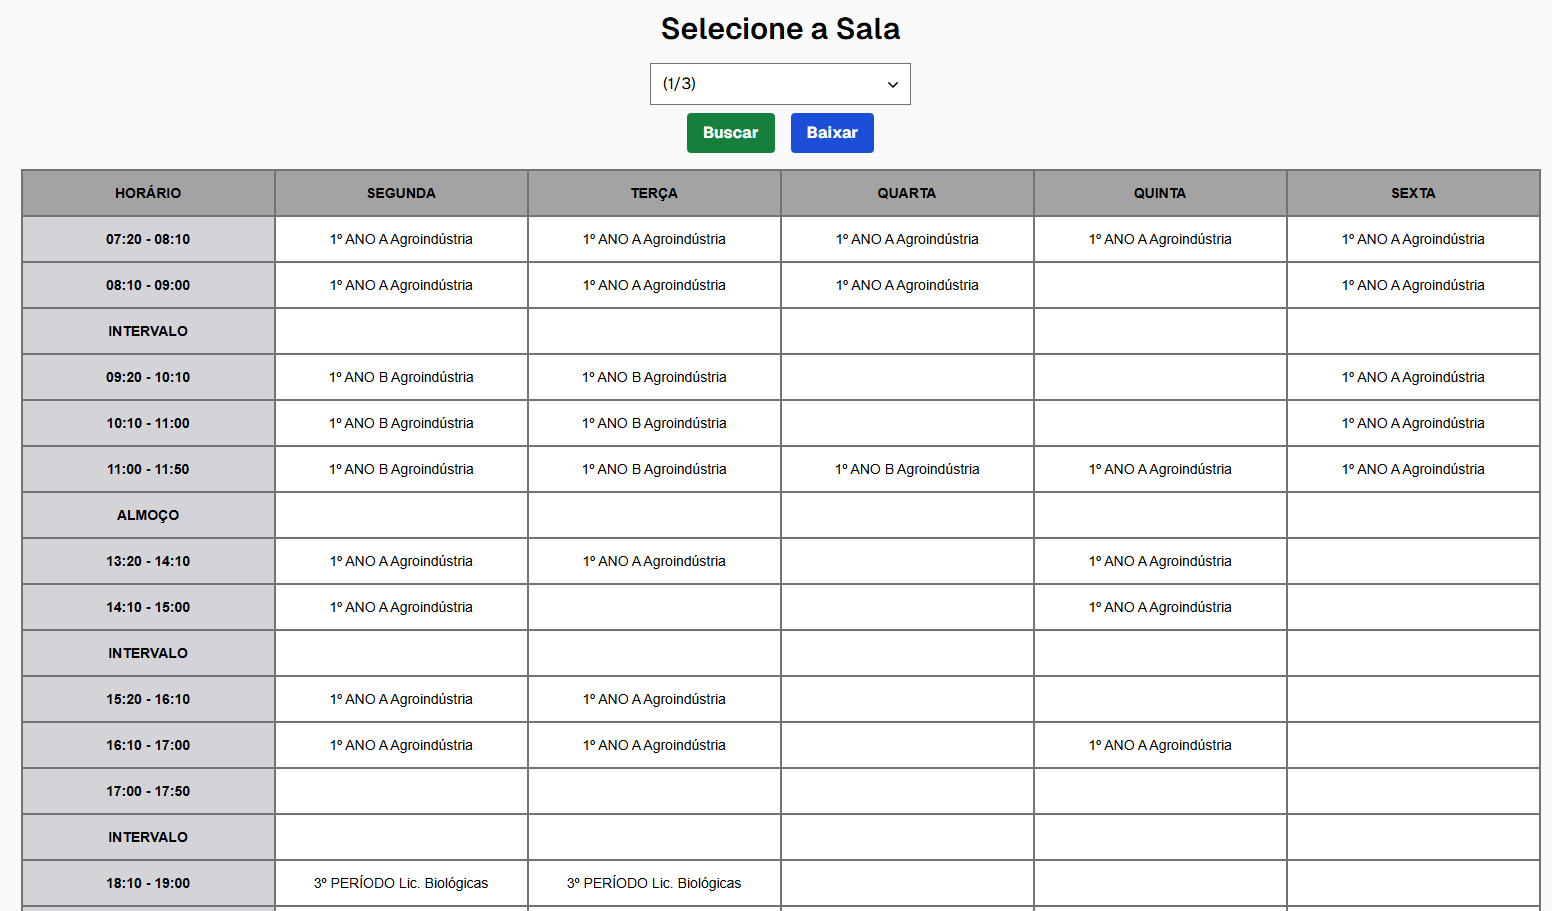
\includegraphics[width=0.8\textwidth]{figuras/front-8.png}
        \\ % Quebra de linha para separar a imagem da fonte
        \small Fonte: Elaborado pelo autor (2025)
    \end{figure}
\end{frame}

\begin{frame}{Desenvolvimento do Front-end}
    \begin{figure}
        \centering
        \vspace{-0.5cm}
        \caption{Tela de login}
        \vspace{-0.2cm}
        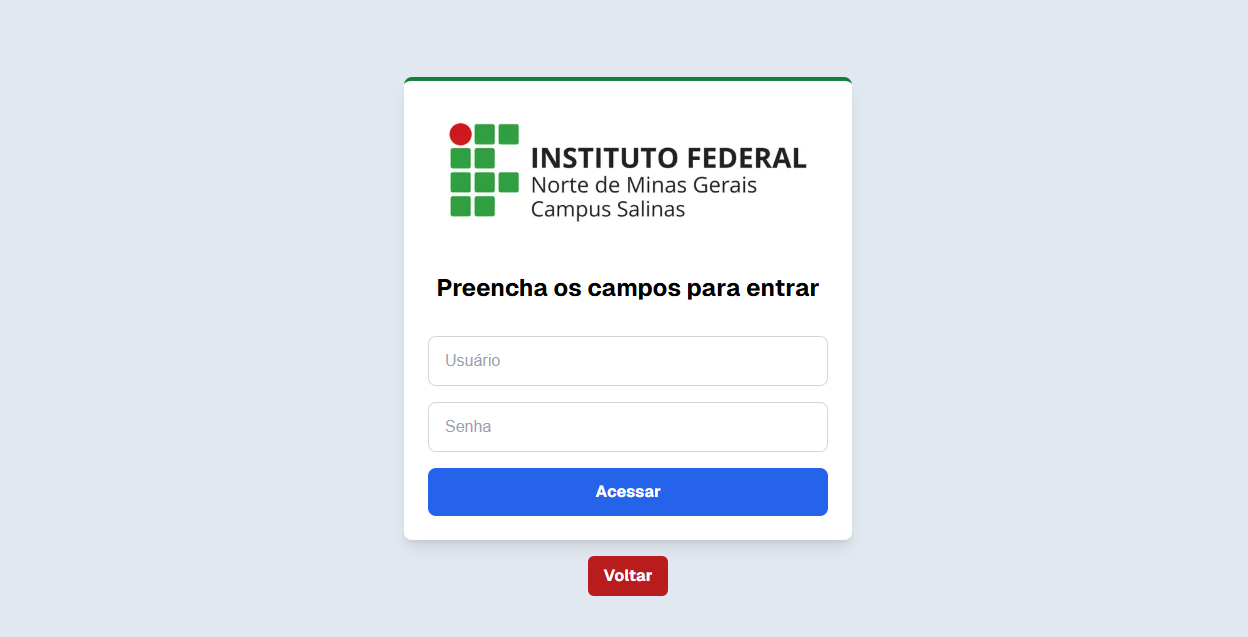
\includegraphics[width=0.8\textwidth]{figuras/front-9.png}
        \\ % Quebra de linha para separar a imagem da fonte
        \small Fonte: Elaborado pelo autor (2025)
    \end{figure}
\end{frame}

\begin{frame}{Desenvolvimento do Front-end}
    \begin{figure}
        \centering
        \vspace{-0.5cm}
        \caption{Tela de validação de dados}
        \vspace{-0.2cm}
        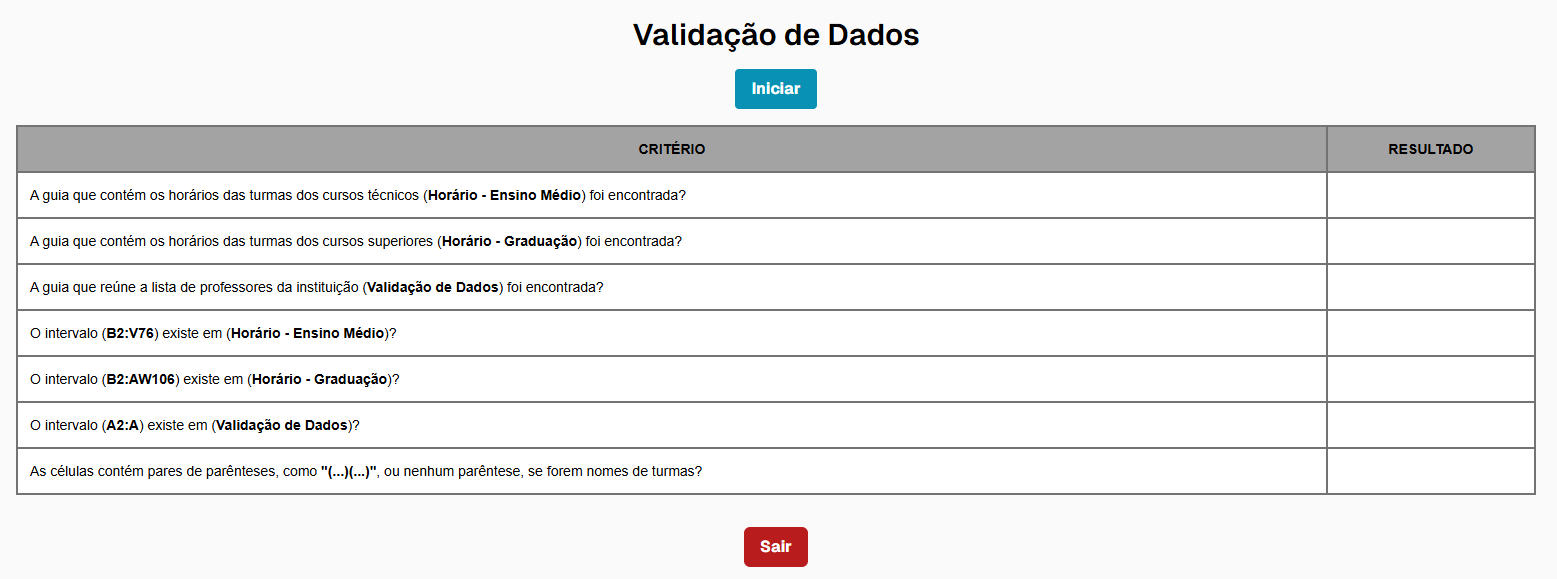
\includegraphics[width=0.8\textwidth]{figuras/front-10.png}
        \\ % Quebra de linha para separar a imagem da fonte
        \small Fonte: Elaborado pelo autor (2025)
    \end{figure}
\end{frame}

\begin{frame}{Desenvolvimento do Front-end}
    \begin{figure}
        \centering
        \vspace{-0.5cm}
        \caption{Sistema que exibe os locais do instituto}
        \vspace{-0.2cm}
        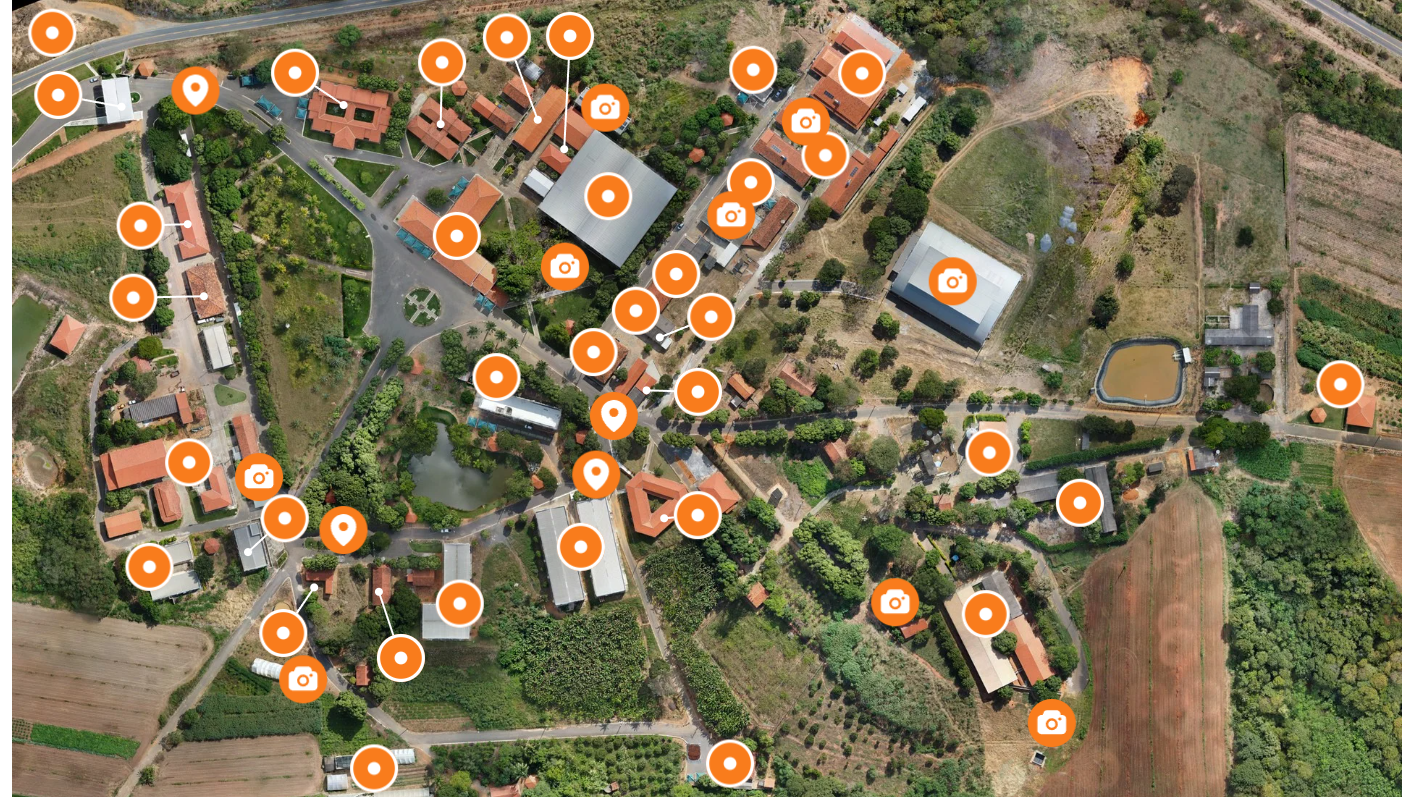
\includegraphics[width=0.8\textwidth]{figuras/front-11.png}
        \\ % Quebra de linha para separar a imagem da fonte
        \small Fonte: Elaborado pelo autor (2025)
    \end{figure}
\end{frame}

\begin{frame}{Desenvolvimento do Front-end}
    \begin{figure}
        \centering
        \vspace{-0.5cm}
        \caption{Sistema de reserva de horários}
        \vspace{-0.2cm}
        
\includegraphics[width=0.8\textwidth]{figuras/front-12.png}
        \\ % Quebra de linha para separar a imagem da fonte
        \small Fonte: Elaborado pelo autor (2025)
    \end{figure}
\end{frame}

\begin{frame}{Desenvolvimento do Front-end}
    \begin{figure}
        \centering
        \vspace{-0.5cm}
        \caption{Sistema de gerenciamento de reserva de salas}
        \vspace{-0.2cm}
        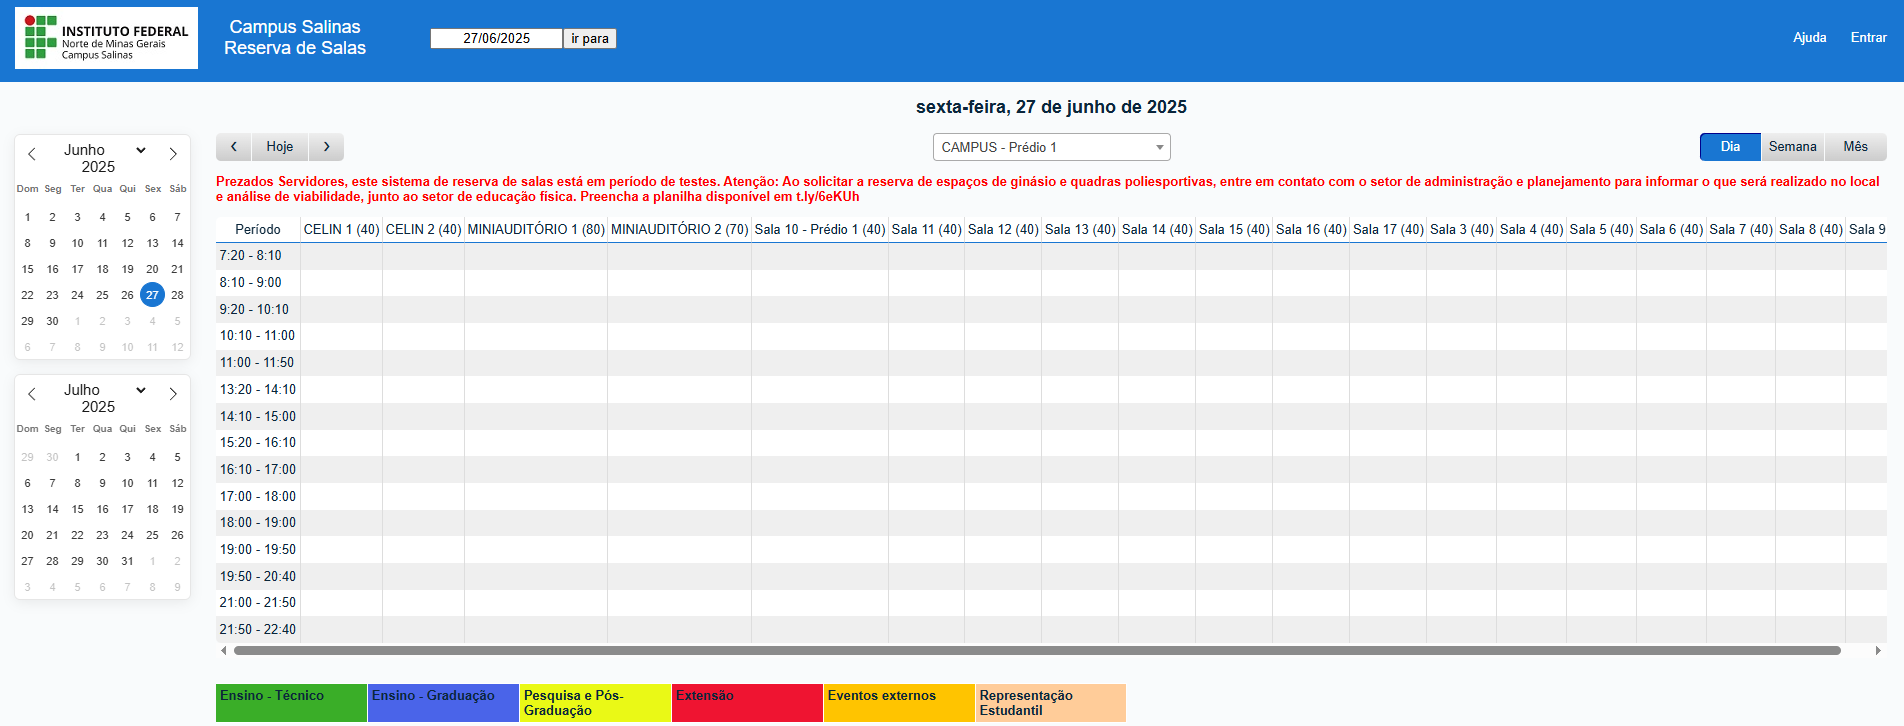
\includegraphics[width=0.8\textwidth]{figuras/front-13.png}
        \\ % Quebra de linha para separar a imagem da fonte
        \small Fonte: Elaborado pelo autor (2025)
    \end{figure}
\end{frame}

\begin{frame}{Estrutura do Front-end}
    \begin{figure}
        \centering
        \vspace{-0.5cm}
        \caption{Estrutura do front-end}
        \vspace{-0.2cm}
        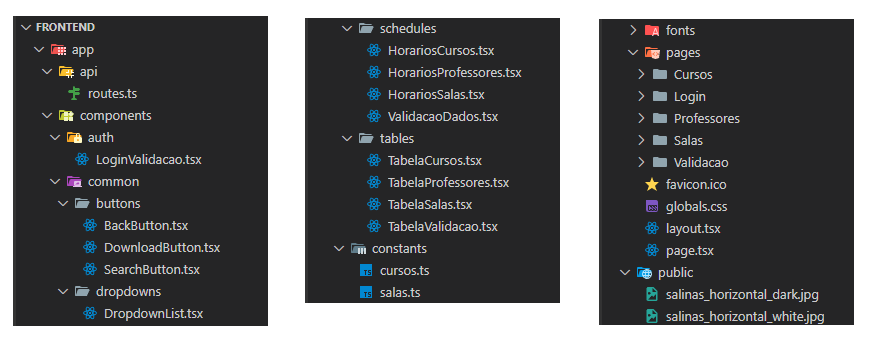
\includegraphics[width=0.6\textwidth]{figuras/front-14.png}
        \\ % Quebra de linha para separar a imagem da fonte
        \small Fonte: Elaborado pelo autor (2025)
    \end{figure}
\end{frame}

\begin{frame}{Funcionalidades do Front-end}
    \begin{figure}
        \centering
        \vspace{-0.5cm}
        \caption{Modo escuro}
        \vspace{-0.2cm}
        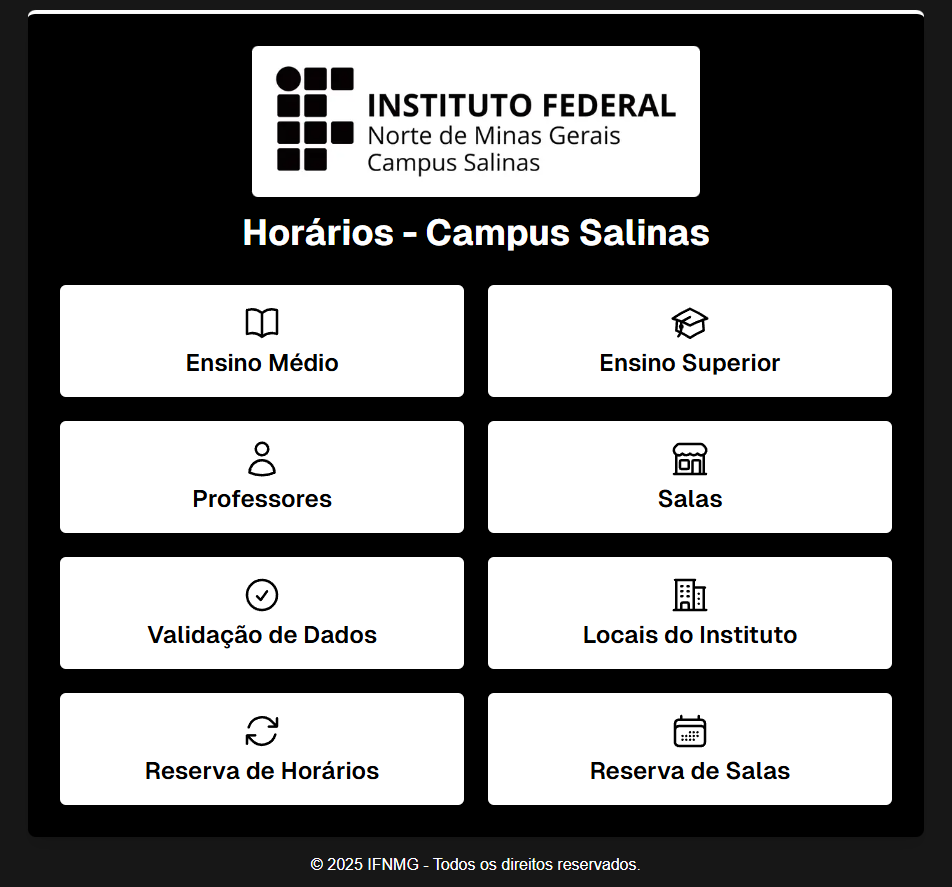
\includegraphics[width=0.6\textwidth]{figuras/front-15.png}
        \\ % Quebra de linha para separar a imagem da fonte
        \small Fonte: Elaborado pelo autor (2025)
    \end{figure}
\end{frame}

\begin{frame}{Funcionalidades do Front-end}
    \begin{figure}
        \centering
        \vspace{-0.5cm}
        \caption{Responsividade}
        \vspace{-0.2cm}
        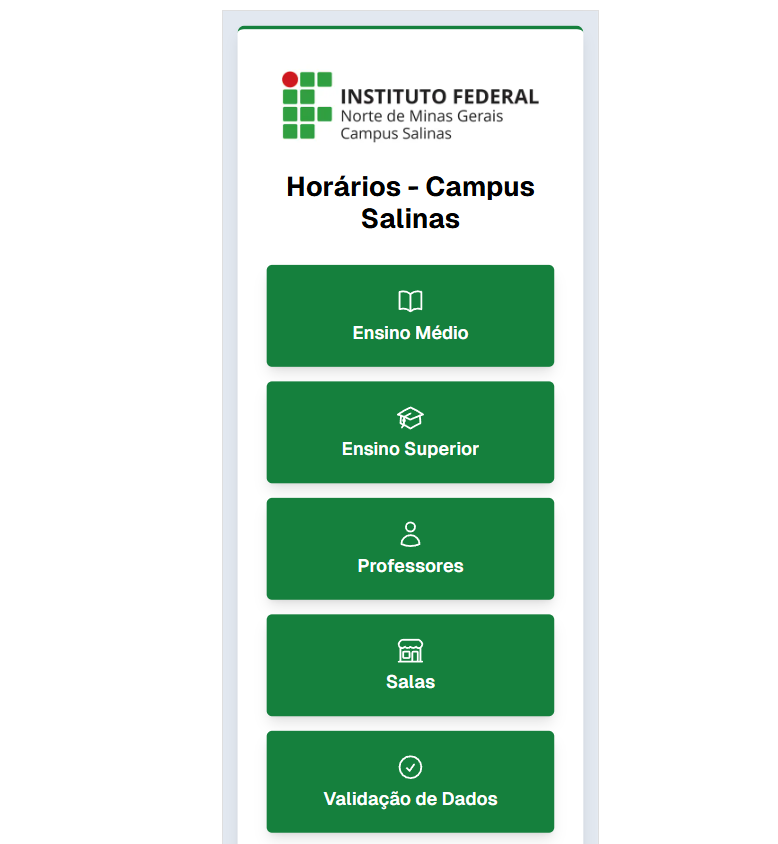
\includegraphics[width=0.5\textwidth]{figuras/front-16.png}
        \\ % Quebra de linha para separar a imagem da fonte
        \small Fonte: Elaborado pelo autor (2025)
    \end{figure}
\end{frame}

\begin{frame}{Funcionalidades do Front-end}
    \begin{figure}
        \centering
        \vspace{-0.5cm}
        \caption{Busca de horários dos cursos técnicos e superiores}
        \vspace{-0.2cm}
        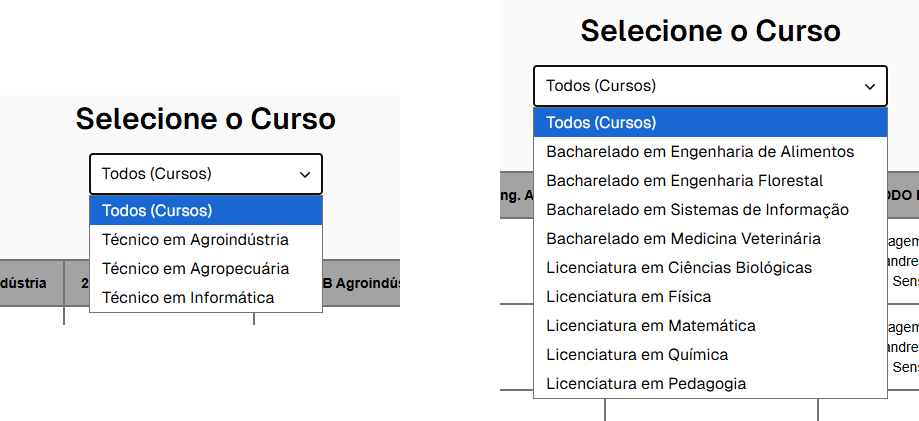
\includegraphics[width=0.7\textwidth]{figuras/front-17.png}
        \\ % Quebra de linha para separar a imagem da fonte
        \small Fonte: Elaborado pelo autor (2025)
    \end{figure}
\end{frame}

\begin{frame}{Funcionalidades do Front-end}
    \begin{figure}
        \centering
        \vspace{-0.5cm}
        \caption{Busca de horários de professores}
        \vspace{-0.2cm}
        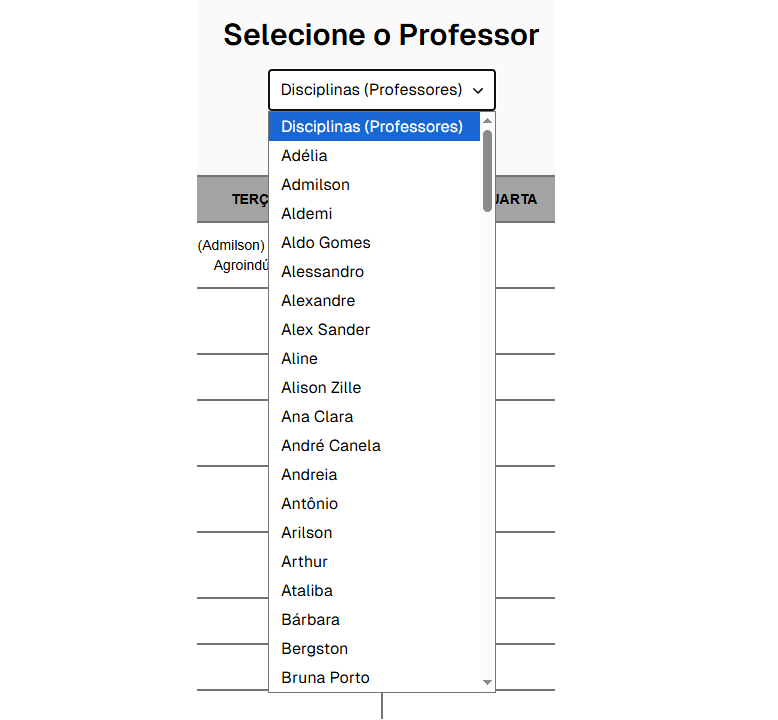
\includegraphics[width=0.6\textwidth]{figuras/front-18.png}
        \\ % Quebra de linha para separar a imagem da fonte
        \small Fonte: Elaborado pelo autor (2025)
    \end{figure}
\end{frame}

\begin{frame}{Funcionalidades do Front-end}
    \begin{figure}
        \centering
        \vspace{-0.5cm}
        \caption{Busca de horários de salas}
        \vspace{-0.2cm}
        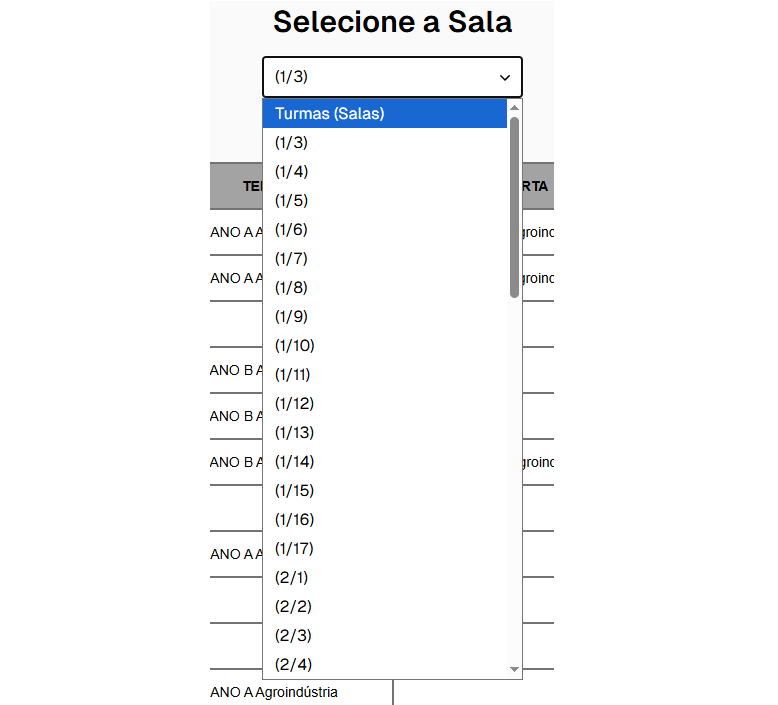
\includegraphics[width=0.6\textwidth]{figuras/front-19.png}
        \\ % Quebra de linha para separar a imagem da fonte
        \small Fonte: Elaborado pelo autor (2025)
    \end{figure}
\end{frame}

\begin{frame}{Funcionalidades do Front-end}
    \begin{figure}
        \centering
        \vspace{-0.5cm}
        \caption{Download em PDF}
        \vspace{-0.2cm}
        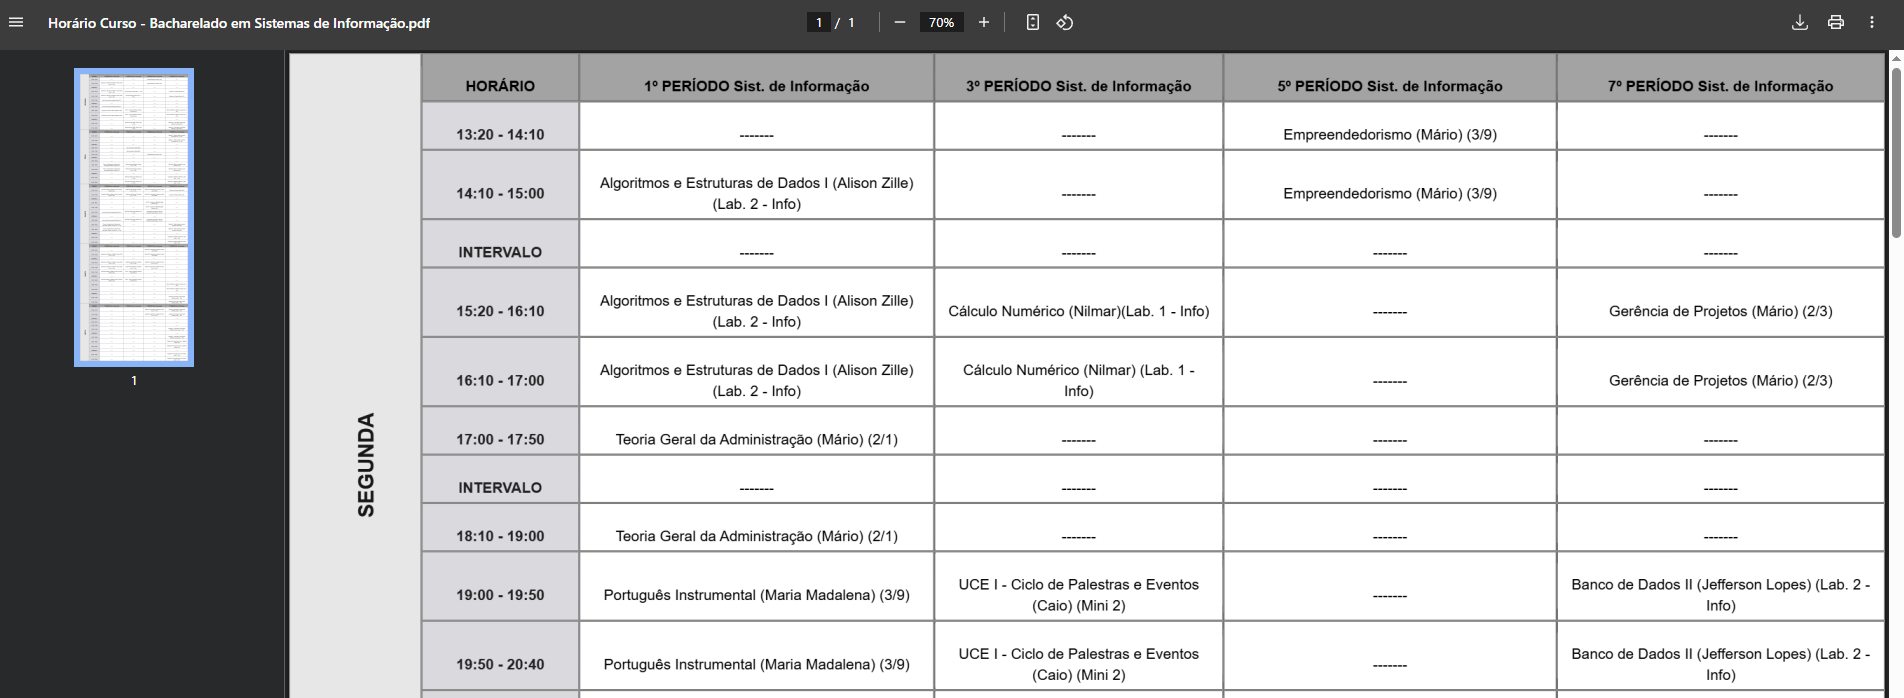
\includegraphics[width=0.9\textwidth]{figuras/front-20.png}
        \\ % Quebra de linha para separar a imagem da fonte
        \small Fonte: Elaborado pelo autor (2025)
    \end{figure}
\end{frame}

\begin{frame}{Funcionalidades do Front-end}
    \begin{figure}
        \centering
        \vspace{-0.5cm}
        \caption{Tela de login com credenciais incorretas}
        \vspace{-0.2cm}
        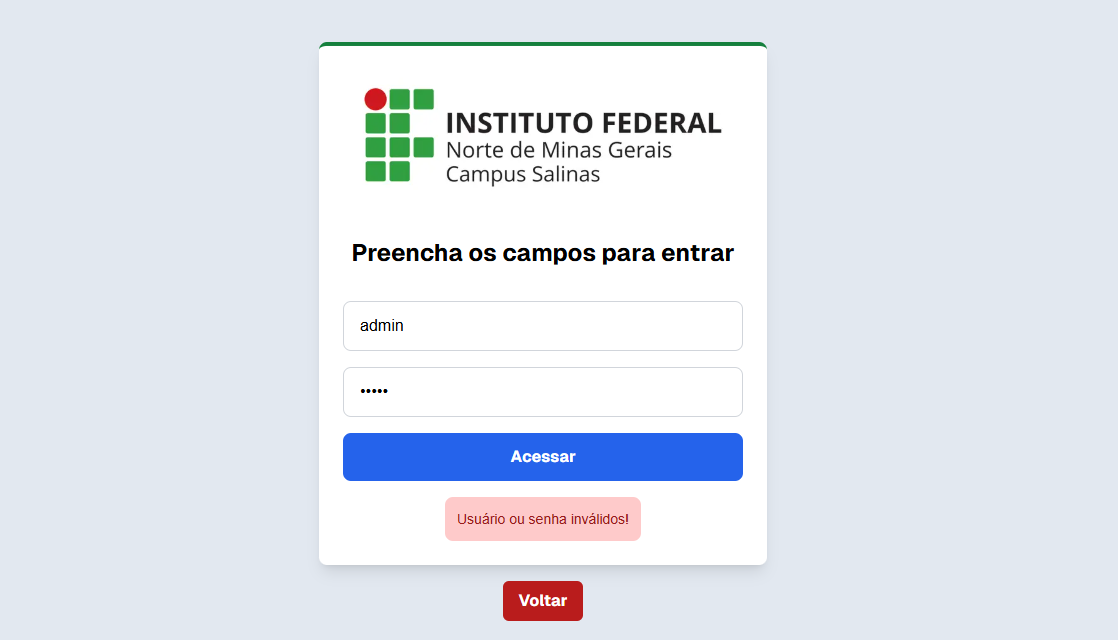
\includegraphics[width=0.8\textwidth]{figuras/front-21.png}
        \\ % Quebra de linha para separar a imagem da fonte
        \small Fonte: Elaborado pelo autor (2025)
    \end{figure}
\end{frame}

\begin{frame}{Funcionalidades do Front-end}
    \begin{figure}
        \centering
        \vspace{-0.5cm}
        \caption{Tela de validação com resultado de sucesso}
        \vspace{-0.2cm}
        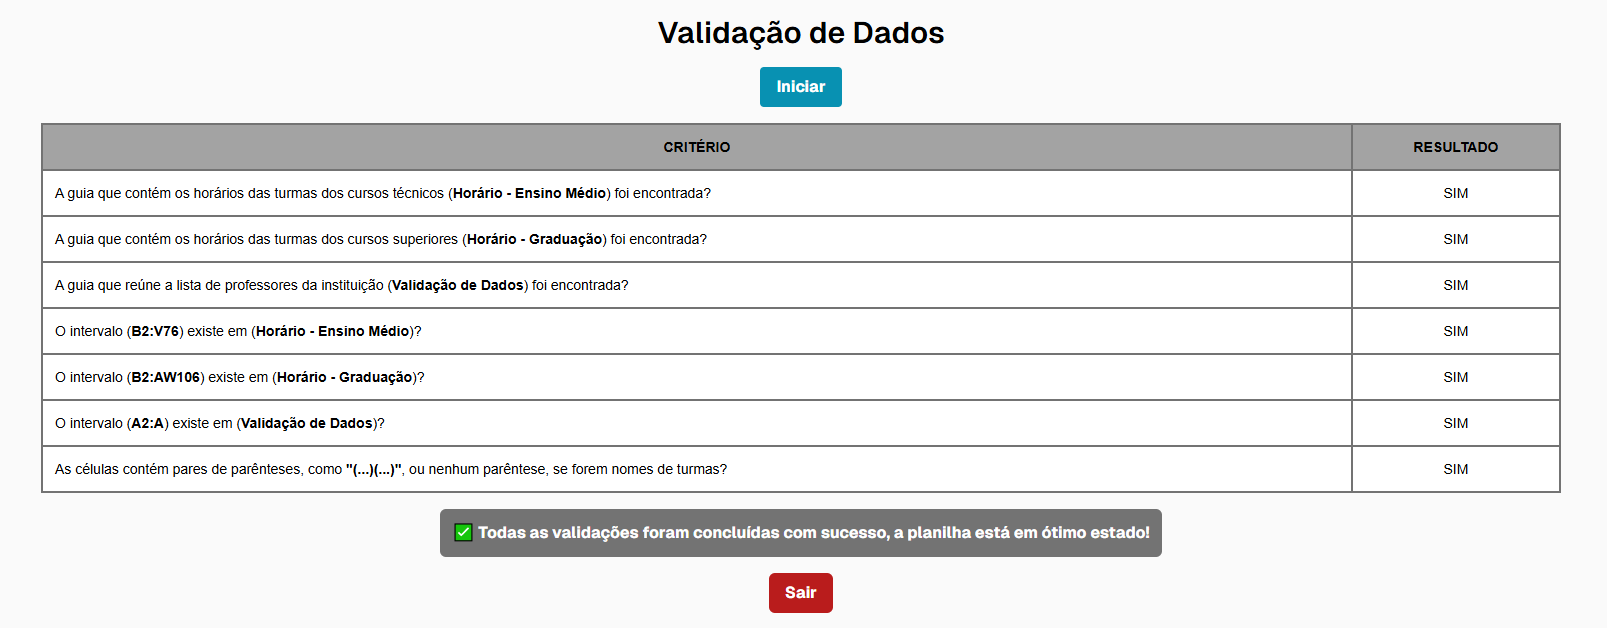
\includegraphics[width=0.8\textwidth]{figuras/front-22.png}
        \\ % Quebra de linha para separar a imagem da fonte
        \small Fonte: Elaborado pelo autor (2025)
    \end{figure}
\end{frame}

\begin{frame}{Funcionalidades do Front-end}
    \begin{figure}
        \centering
        \vspace{-0.5cm}
        \caption{Tela de validação com resultado mostrando inconsistências}
        \vspace{-0.2cm}
        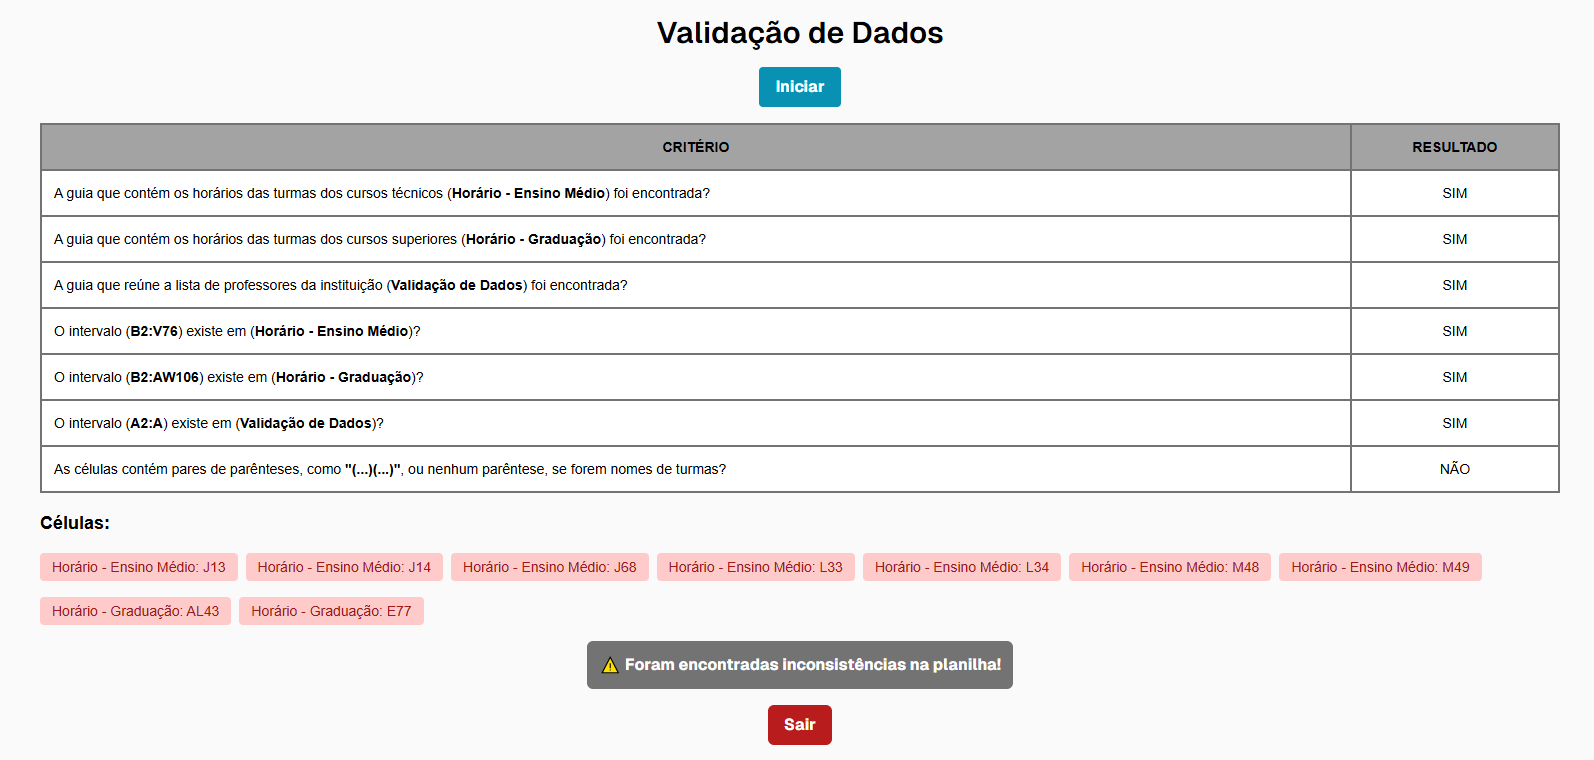
\includegraphics[width=0.8\textwidth]{figuras/front-23.png}
        \\ % Quebra de linha para separar a imagem da fonte
        \small Fonte: Elaborado pelo autor (2025)
    \end{figure}
\end{frame}

\begin{frame}{Funcionalidades do Front-end}
    \begin{figure}
        \centering
        \vspace{-0.5cm}
        \caption{Tela de validação com resultado de erro}
        \vspace{-0.2cm}
        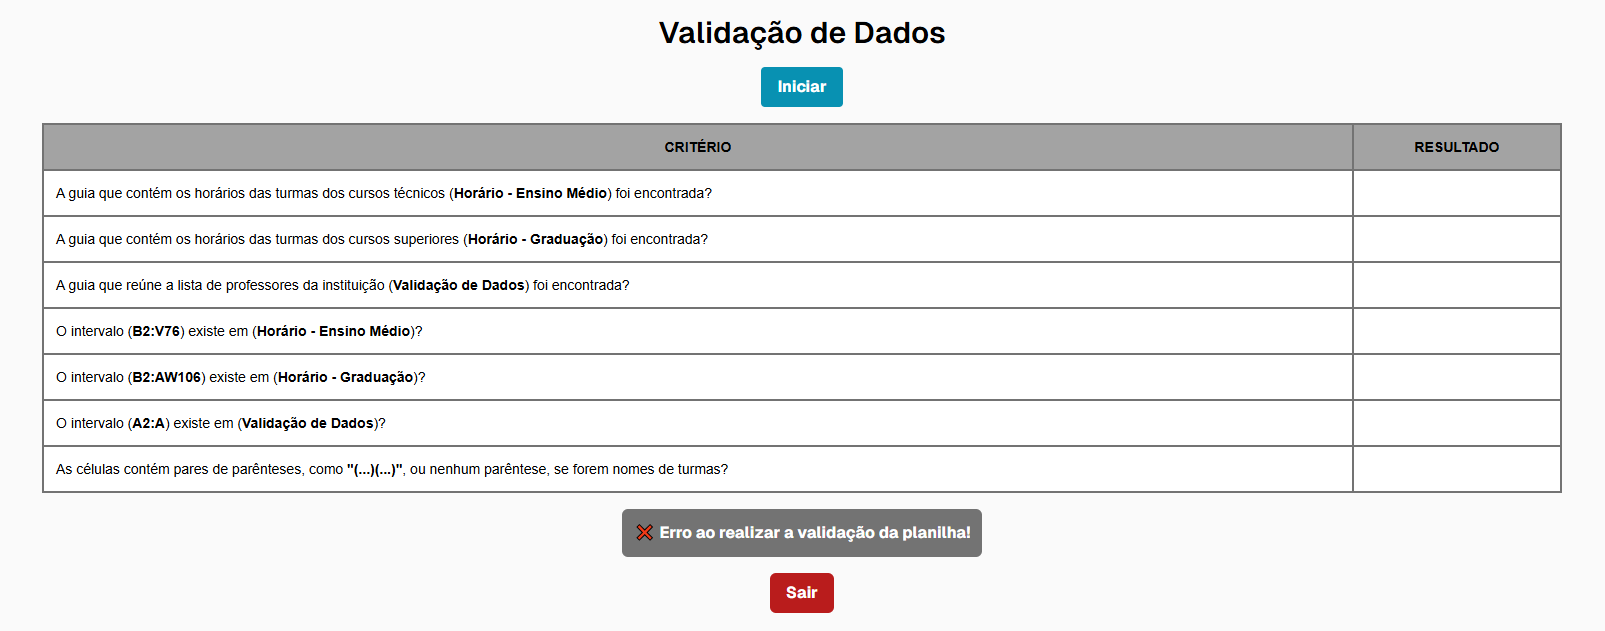
\includegraphics[width=0.8\textwidth]{figuras/front-24.png}
        \\ % Quebra de linha para separar a imagem da fonte
        \small Fonte: Elaborado pelo autor (2025)
    \end{figure}
\end{frame}

\begin{frame}{Back-end}
    \begin{itemize}
		\item Google Sheets como Banco de Dados: \vspace{0.5cm}
	\end{itemize}
    \begin{figure}
        \centering
        \vspace{-0.8cm}
        \caption{Guia ``Horário - Ensino Médio''}
        \vspace{-0.2cm}
        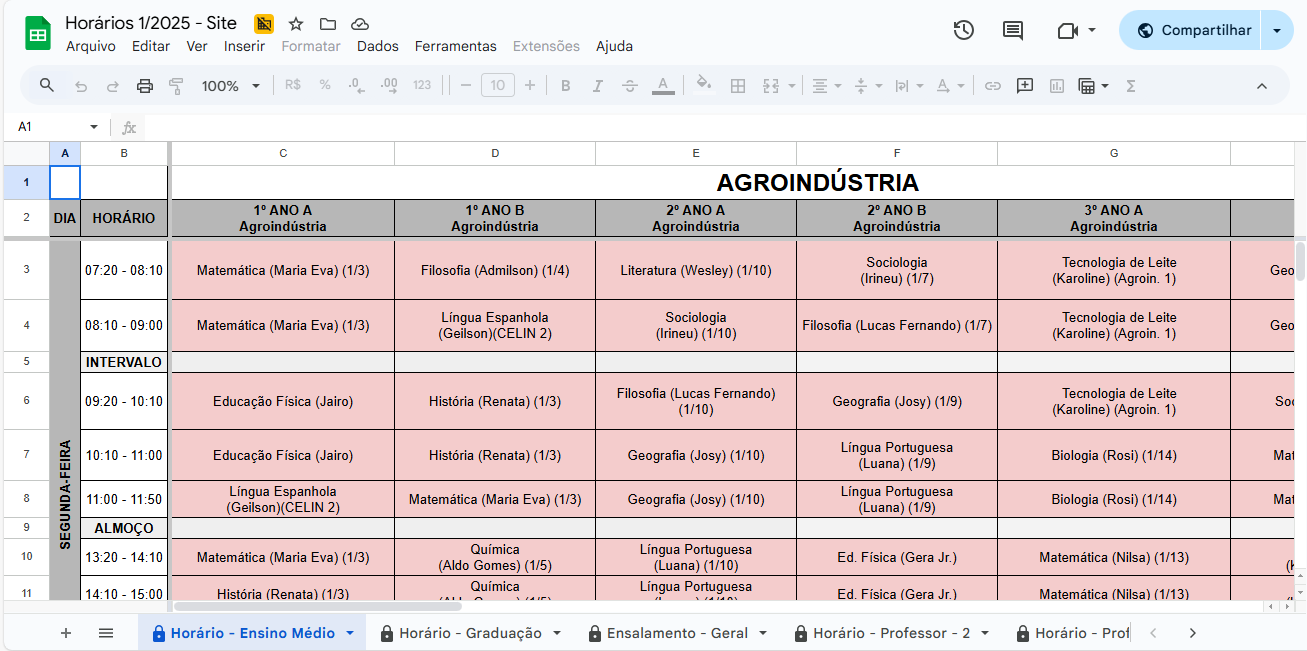
\includegraphics[width=0.8\textwidth]{figuras/plan-1.png}
        \\ % Quebra de linha para separar a imagem da fonte
        \small Fonte: Elaborado pelo autor (2025)
    \end{figure}
\end{frame}

\begin{frame}{Google Sheets como Banco de Dados}
    \begin{figure}
        \centering
        \vspace{-0.5cm}
        \caption{Guia ``Horário - Graduação''}
        \vspace{-0.2cm}
        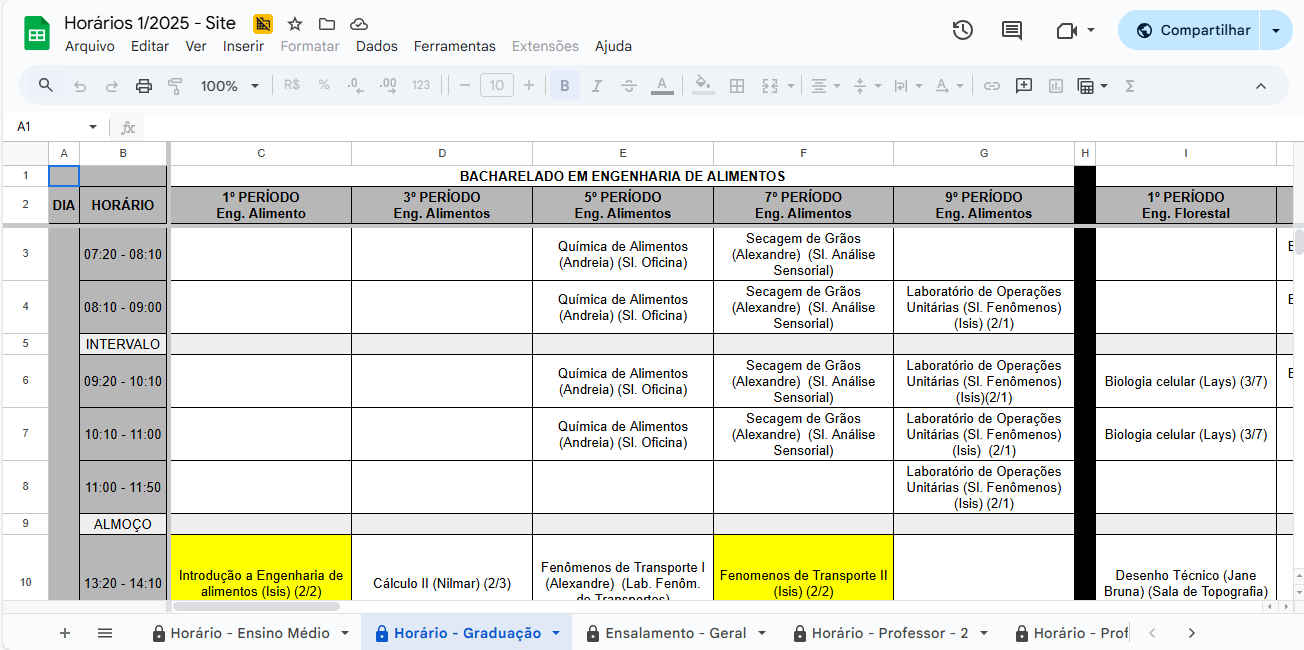
\includegraphics[width=0.8\textwidth]{figuras/plan-2.png}
        \\ % Quebra de linha para separar a imagem da fonte
        \small Fonte: Elaborado pelo autor (2025)
    \end{figure}
\end{frame}

\begin{frame}{Google Sheets como Banco de Dados}
    \begin{figure}
        \centering
        \vspace{-0.5cm}
        \caption{Guia ``Validação de Dados''}
        \vspace{-0.2cm}
        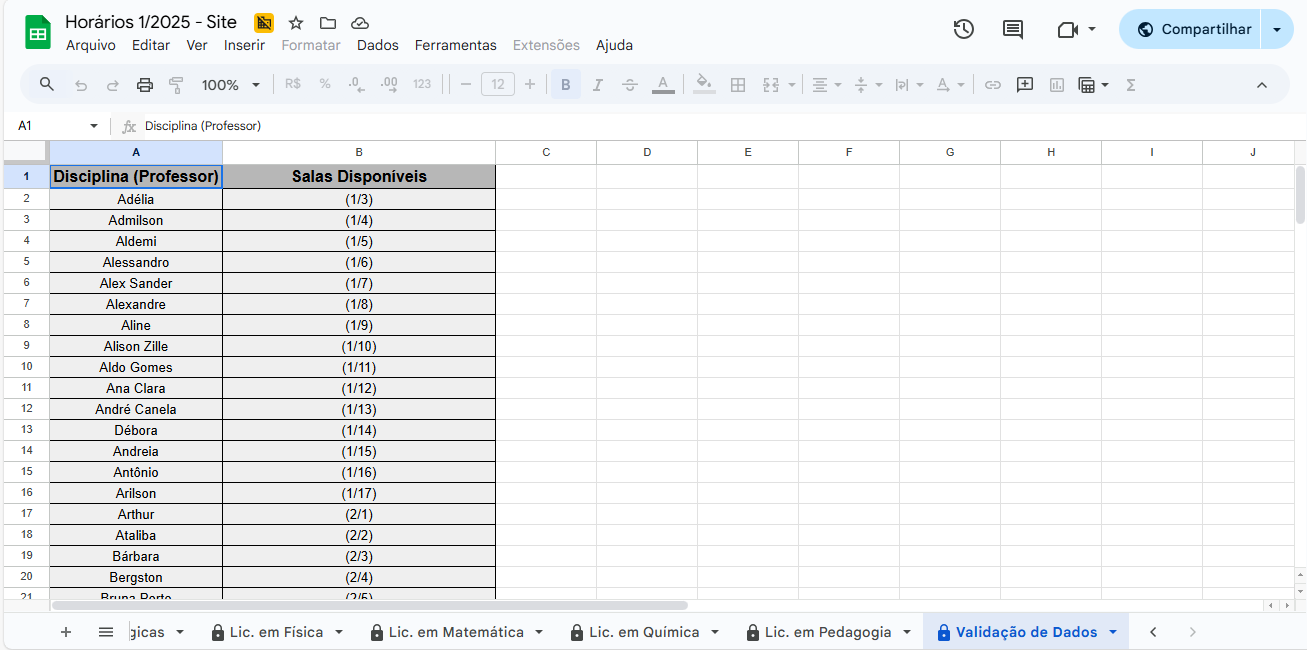
\includegraphics[width=0.8\textwidth]{figuras/plan-3.png}
        \\ % Quebra de linha para separar a imagem da fonte
        \small Fonte: Elaborado pelo autor (2025)
    \end{figure}
\end{frame}

\begin{frame}{Google Sheets como Banco de Dados}
    \begin{figure}
        \centering
        \vspace{-0.5cm}
        \caption{Guia ``Login''}
        \vspace{-0.2cm}
        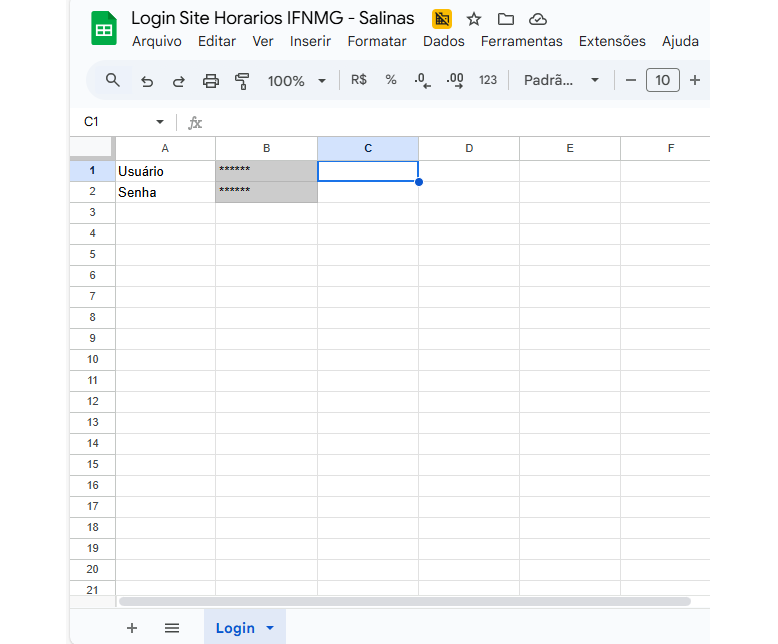
\includegraphics[width=0.6\textwidth]{figuras/plan-4.png}
        \\ % Quebra de linha para separar a imagem da fonte
        \small Fonte: Elaborado pelo autor (2025)
    \end{figure}
\end{frame}

\begin{frame}{Estrutura do Back-end}
    \begin{figure}
        \centering
        \vspace{-0.5cm}
        \caption{Estrutura do back-end}
        \vspace{-0.2cm}
        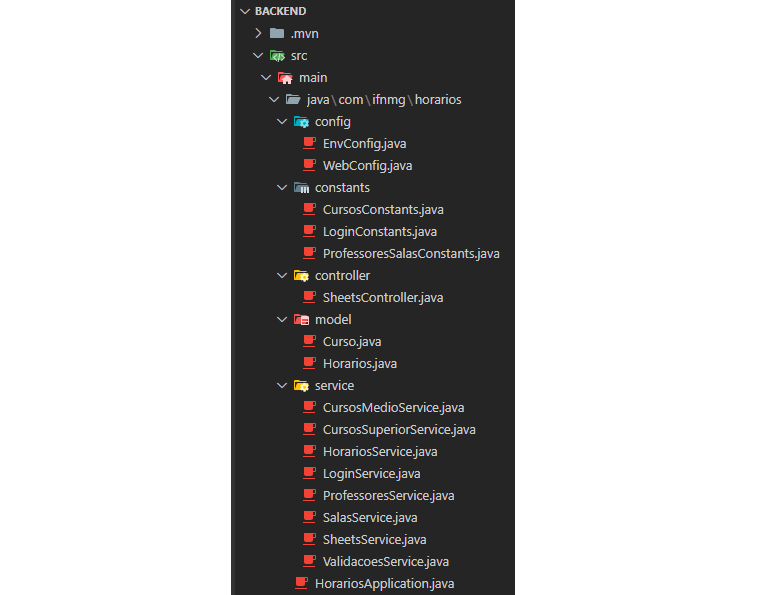
\includegraphics[width=0.7\textwidth]{figuras/back-1.png}
        \\ % Quebra de linha para separar a imagem da fonte
        \small Fonte: Elaborado pelo autor (2025)
    \end{figure}
\end{frame}

\begin{frame}{Funcionalidades do Back-end}
    \begin{itemize}
		\item Estabelecer a conexão com a API do Google Sheets
	\end{itemize}
    \begin{figure}
        \centering
        \vspace{-0.5cm}
        \caption{Classe ``SheetsService.java''}
        \vspace{-0.2cm}
        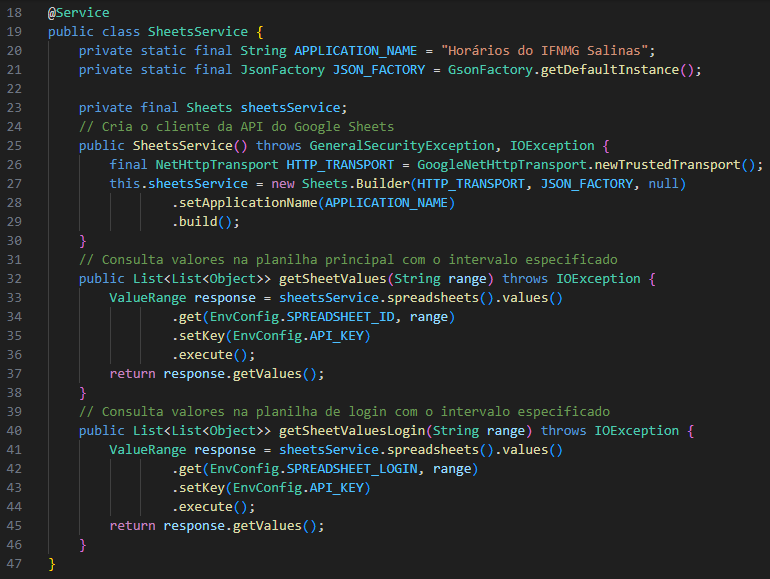
\includegraphics[width=0.6\textwidth]{figuras/back-2.png}
        \\ % Quebra de linha para separar a imagem da fonte
        \small Fonte: Elaborado pelo autor (2025)
    \end{figure}
\end{frame}

\begin{frame}{Funcionalidades do Back-end}
    \begin{itemize}
		\item Disponibilizar endpoints REST
	\end{itemize}
    \begin{figure}
        \centering
        \vspace{-0.3cm}
        \caption{Endpoint de consulta dos horários dos cursos técnicos}
        \vspace{-0.2cm}
        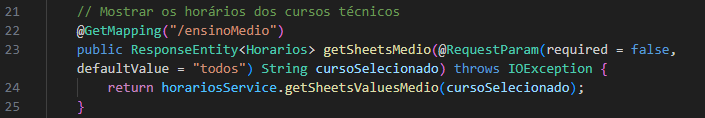
\includegraphics[width=0.7\textwidth]{figuras/back-3.png}
        \\ % Quebra de linha para separar a imagem da fonte
        \small Fonte: Elaborado pelo autor (2025)
    \end{figure}
    \begin{figure}
        \centering
        \vspace{-0.5cm}
        \caption{Endpoint de consulta dos horários dos cursos superiores}
        \vspace{-0.2cm}
        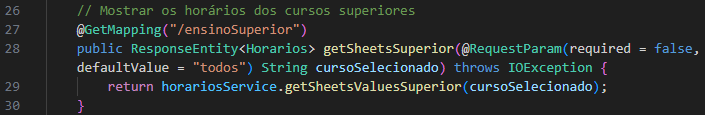
\includegraphics[width=0.7\textwidth]{figuras/back-4.png}
        \\ % Quebra de linha para separar a imagem da fonte
        \small Fonte: Elaborado pelo autor (2025)
    \end{figure}
\end{frame}

\begin{frame}{Funcionalidades do Back-end}
    \begin{figure}
        \centering
        \vspace{-0.3cm}
        \caption{Endpoint de consulta dos horários dos professores}
        \vspace{-0.2cm}
        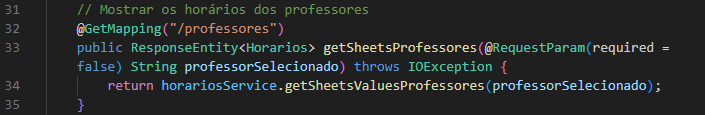
\includegraphics[width=0.7\textwidth]{figuras/back-5.png}
        \\ % Quebra de linha para separar a imagem da fonte
        \small Fonte: Elaborado pelo autor (2025)
    \end{figure}
    \begin{figure}
        \centering
        \vspace{-0.5cm}
        \caption{Endpoint de consulta dos horários de ocupação das salas}
        \vspace{-0.2cm}
        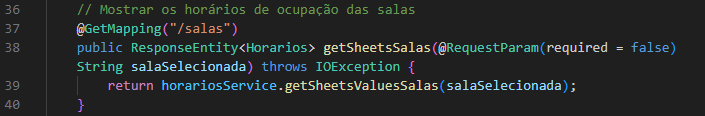
\includegraphics[width=0.7\textwidth]{figuras/back-6.png}
        \\ % Quebra de linha para separar a imagem da fonte
        \small Fonte: Elaborado pelo autor (2025)
    \end{figure}
\end{frame}

\begin{frame}{Funcionalidades do Back-end}
    \begin{figure}
        \centering
        \vspace{-0.3cm}
        \caption{Endpoint de consulta das permissões para visualizar validação da planiha}
        \vspace{-0.2cm}
        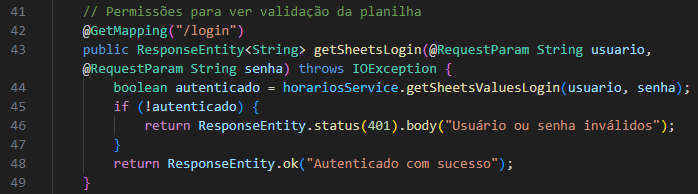
\includegraphics[width=0.7\textwidth]{figuras/back-7.png}
        \\ % Quebra de linha para separar a imagem da fonte
        \small Fonte: Elaborado pelo autor (2025)
    \end{figure}
    \begin{figure}
        \centering
        \vspace{-0.5cm}
        \caption{Endpoint de consulta para validar dados da planilha}
        \vspace{-0.2cm}
        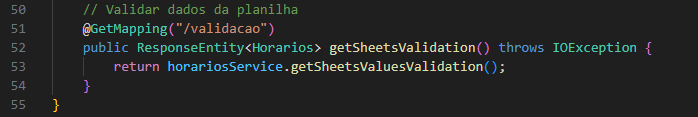
\includegraphics[width=0.7\textwidth]{figuras/back-8.png}
        \\ % Quebra de linha para separar a imagem da fonte
        \small Fonte: Elaborado pelo autor (2025)
    \end{figure}
\end{frame}

\begin{frame}{Deploy}
    \begin{itemize}
		\item Front-end:
	\end{itemize}
    \begin{figure}
        \centering
        \vspace{-0.3cm}
        \caption{Deploy do front-end da plataforma na Vercel}
        \vspace{-0.2cm}
        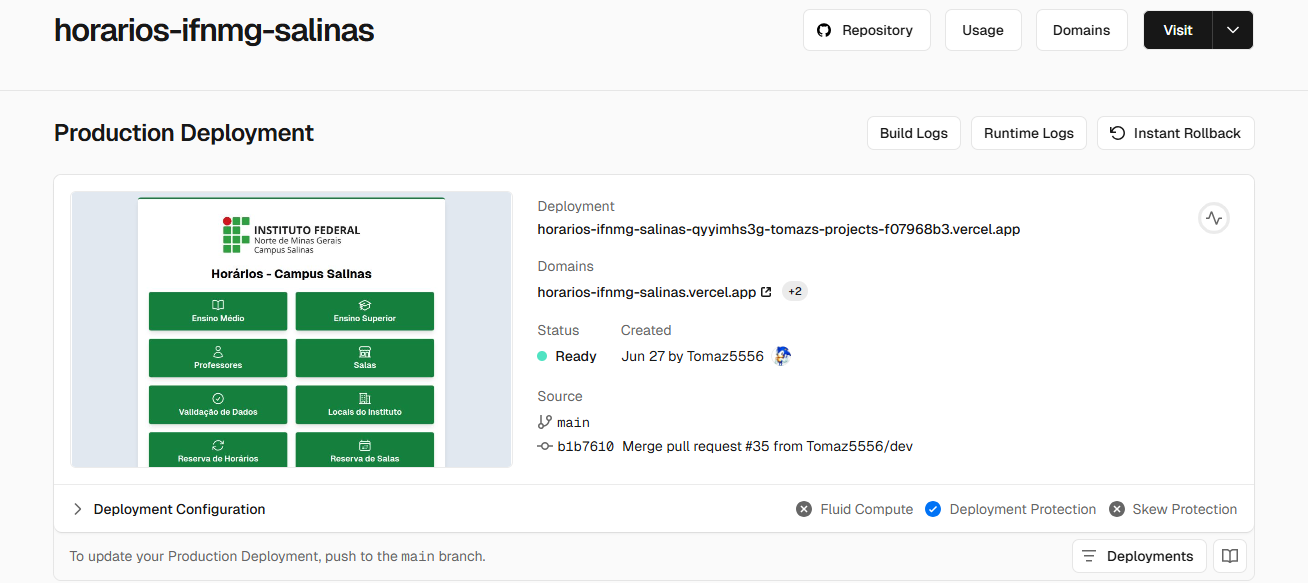
\includegraphics[width=0.7\textwidth]{figuras/deploy-1.png}
        \\ % Quebra de linha para separar a imagem da fonte
        \small Fonte: Elaborado pelo autor (2025)
    \end{figure}
\end{frame}

\begin{frame}{Deploy}
    \begin{itemize}
		\item Back-end:
	\end{itemize}
    \begin{figure}
        \centering
        \vspace{-0.3cm}
        \caption{Deploy do back-end da plataforma na Koyeb}
        \vspace{-0.2cm}
        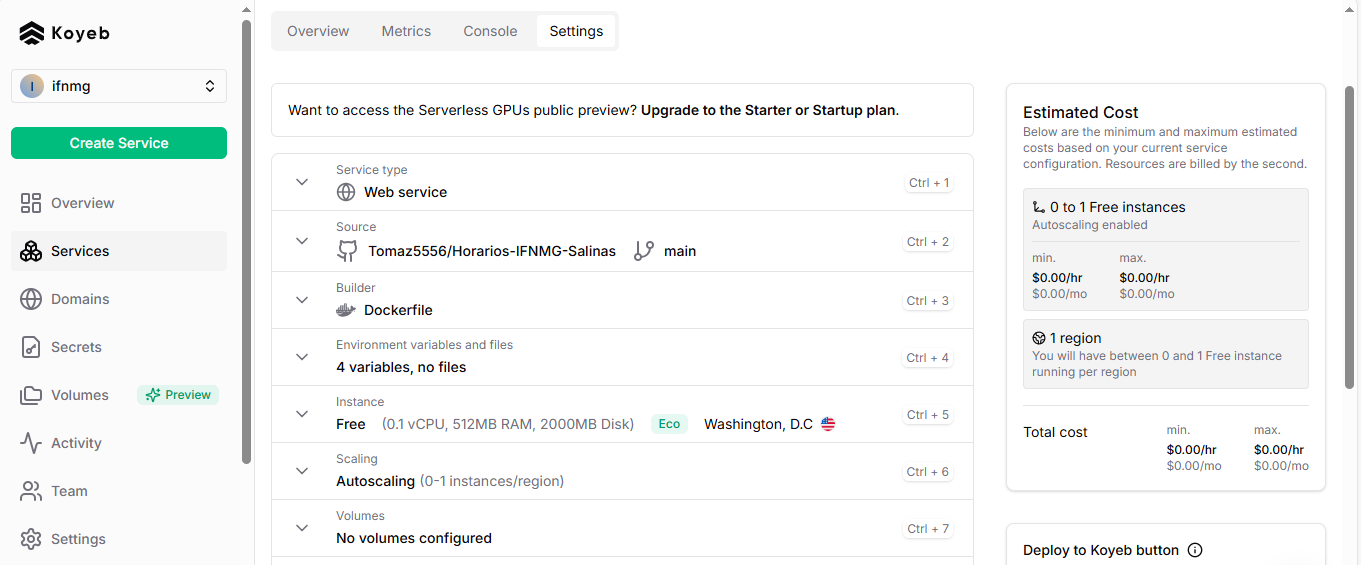
\includegraphics[width=0.7\textwidth]{figuras/deploy-2.png}
        \\ % Quebra de linha para separar a imagem da fonte
        \small Fonte: Elaborado pelo autor (2025)
    \end{figure}
\end{frame}

\begin{frame}{Documentação}
    \begin{itemize}
		\item Documentação técnica elaborada para a planilha utilizada como banco de dados do sistema.
	\end{itemize}
    \begin{figure}
        \centering
        \vspace{-0.3cm}
        \caption{Instruções para desenvolvedores}
        \vspace{-0.2cm}
        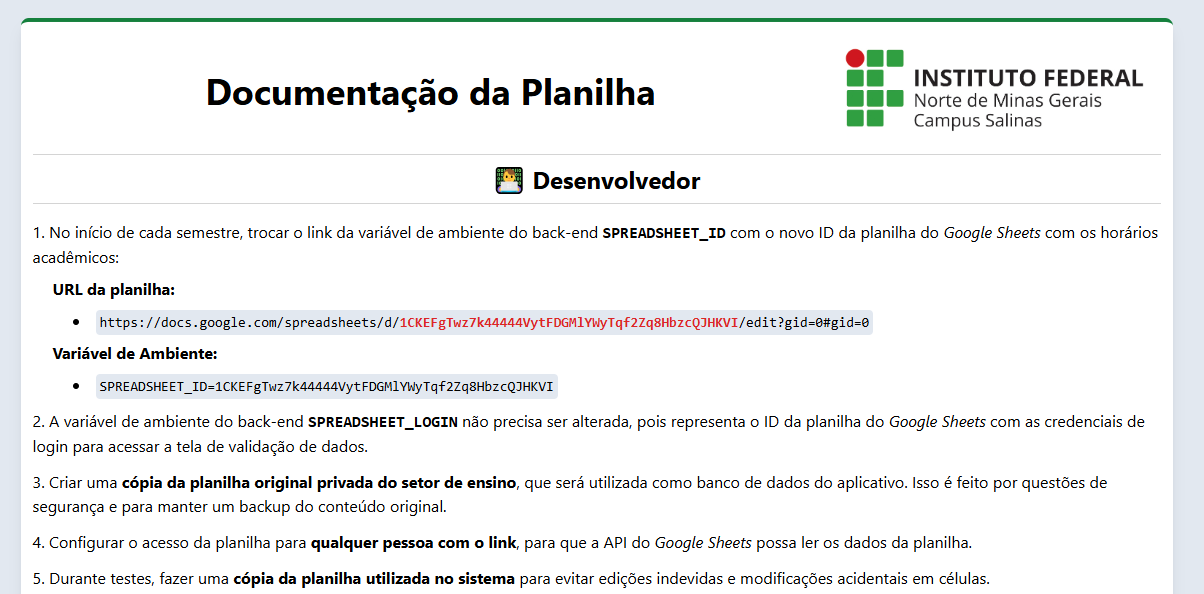
\includegraphics[width=0.7\textwidth]{figuras/doc-1.png}
        \\ % Quebra de linha para separar a imagem da fonte
        \small Fonte: Elaborado pelo autor (2025)
    \end{figure}
\end{frame}

\begin{frame}{Documentação}
    \begin{figure}
        \centering
        \vspace{-0.3cm}
        \caption{Instruções para administradores da planilha}
        \vspace{-0.2cm}
        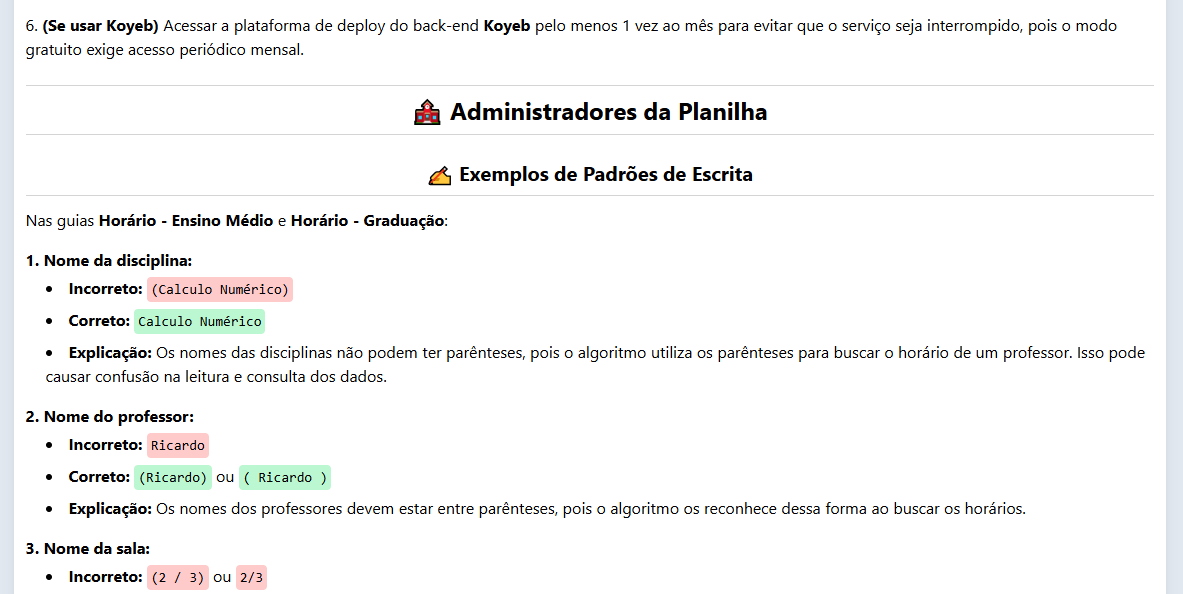
\includegraphics[width=0.7\textwidth]{figuras/doc-2.png}
        \\ % Quebra de linha para separar a imagem da fonte
        \small Fonte: Elaborado pelo autor (2025)
    \end{figure}
\end{frame}

\begin{frame}{Documentação}
    \begin{figure}
        \centering
        \vspace{-0.3cm}
        \caption{Explicação das guias e intervalos de células}
        \vspace{-0.2cm}
        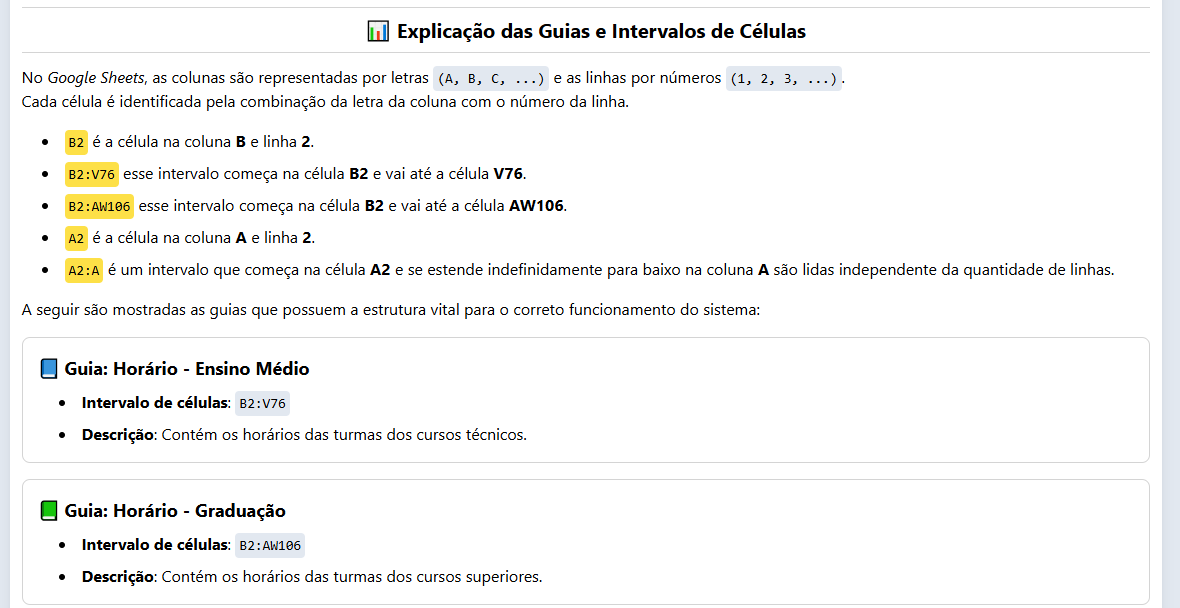
\includegraphics[width=0.7\textwidth]{figuras/doc-3.png}
        \\ % Quebra de linha para separar a imagem da fonte
        \small Fonte: Elaborado pelo autor (2025)
    \end{figure}
\end{frame}

\begin{frame}{Documentação}
    \begin{figure}
        \centering
        \vspace{-0.3cm}
        \caption{Observação sobre mudanças estruturais}
        \vspace{-0.2cm}
        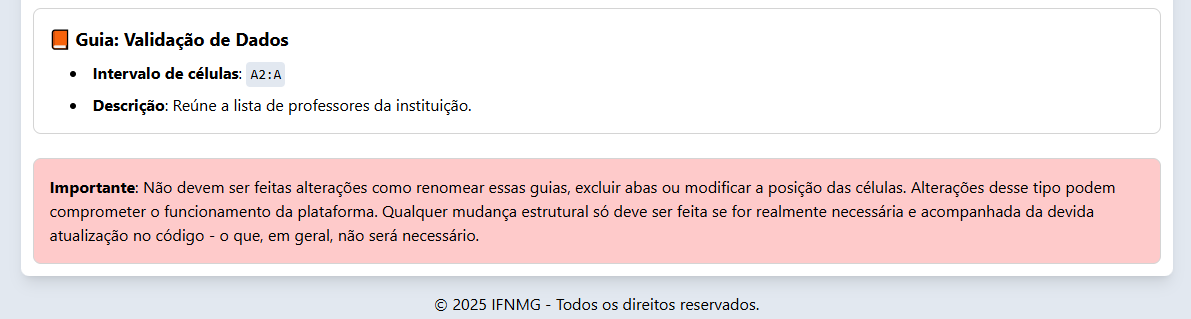
\includegraphics[width=0.7\textwidth]{figuras/doc-4.png}
        \\ % Quebra de linha para separar a imagem da fonte
        \small Fonte: Elaborado pelo autor (2025)
    \end{figure}
\end{frame}

\section{Conclusão}

\begin{frame}{Conclusão}
    \begin{itemize}
        \item Objetivo do Projeto; \vspace{0.5cm}
        \item Abordagem da Solução; \vspace{0.5cm}
        \item Relevância e Contribuições; \vspace{0.5cm}
        \item Resultados Alcançados; \vspace{0.5cm}
        \item Limitações; \vspace{0.5cm}
        \item Trabalhos Futuros. \vspace{0.5cm}
    \end{itemize}
\end{frame}



% Referencias
%\include{tex/referencias/referencias}

% Agradecimentos
\section{}
\begin{frame}{Agradecimentos}
	\begin{itemize}
		\item Antes de tudo, agradeço a Deus, por me conceder força e sabedoria ao longo da jornada; \vspace{0.5cm}
		\item Sou grato à minha família pelo apoio incondicional e aos colegas de curso pela parceria e colaboração; \vspace{0.5cm}
		\item Ao professor Leonardo, pela orientação no desenvolvimento deste trabalho e por compartilhar seus conhecimentos; \vspace{0.5cm}
		\item Ao professor Frederico, pela orientação durante a bolsa treinamento e pelas contribuições na compreensão da gestão dos horários acadêmicos do campus. \vspace{0.5cm}
	\end{itemize}
\end{frame}

\begin{frame}{Contato}
	\begin{itemize}
		\item Github: \url{https://github.com/Tomaz5556} \vspace{0.5cm}
		\item Facebook: \url{https://www.facebook.com/tomaz.5556} \vspace{0.5cm}
		\item Discord: \url{https://discord.com/users/1157463246027096215} \vspace{0.5cm}
		\item Whatsapp: (38984263205) \vspace{0.5cm}
	\end{itemize}
\end{frame}

\end{document}